\chapter{Improve the Radial Velocity Precision of HET/HRS}\label{chap:het}

This is about HET/HRS. This will have introduction to HET and HRS.

%%%%%%%%%%%%%%%%%%%%%%%%%%%%%%%%%%%%%%%%%%%%%%%%%%%%%%%%%%%%%%%%%%%%%%%%%%%%%%
\section{Adoption of REDUCE and the CPS Doppler Code for HET/HRS}


%----------------------------------------------------------------
% HD 37605 and the improvement on precision brought by temperature stabilization
% plot made by ~/ExoPlanet-2010-2011/Targets/37605/rv_plot/rvplot_NESSF2013.eps
% grabbed from ~/ExoPlanet-2010-2011/Professional_Development/201301-NESSF/proposal/
\begin{figure}
\centering
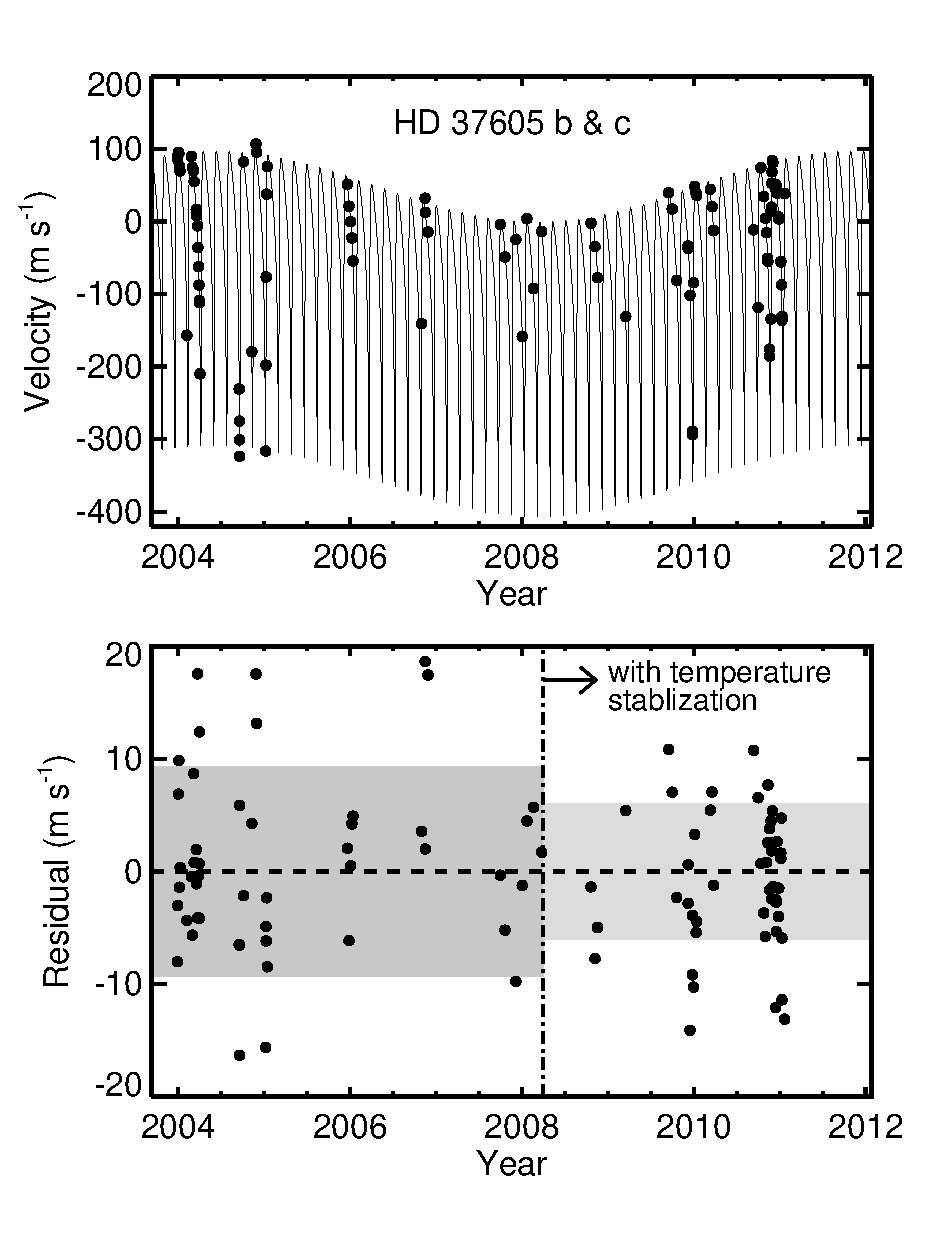
\includegraphics[scale=0.5]{het/37605.eps}
\caption{Illustration of the effects of temperature stabilization on
  \het\ RV precision, using data on the HD~37605 system (see
  Chapter~\ref{chap:planets}). The RMS of the RV residuals (bottom
  panel) against the best-fit two-planet Keplerian solution (solid
  line in top panel) has dropped from 9~m/s to 6~m/s (grey areas in
  the bottom plot) after implementation of fine temperature control in
  the spectrograph room in March 2008. The pre-2009 \het\ data are
  provided by the UT Austin group.
\label{het:fig:tempstable}}
\end{figure}
%----------------------------------------------------------------





%%%%%%%%%%%%%%%%%%%%%%%%%%%%%%%%%%%%%%%%%%%%%%%%%%%%%%%%%%%%%%%%%%%%%%%%%%%%%%
\section{The Search for a Better Instrumental Profile}\label{het:sec:ip}

% HET IP section

Finding a good customized function for the instrumental profile (IP)
for a precise RV spectrograph is undoubtedly one of the most important
and difficult tasks in achieving a $<3$~m/s RV precision. IP modeling
is a crucial part of the precise RV work with iodine calibration, as
it affects directly several key procedures in the Doppler pipeline,
such as the creation of stellar spectrum template and the
forward-modeling of the observed stellar$+$iodine spectrum. The heroic
efforts of early \keck\ users pinned down its IP to a 12-parameter
sum-of-Gaussians profile, with two sets of 11 pre-determined positions
and width of the satellite Gaussians \citep{1995PASP..107..966V}. It
is the product of careful studies and numerous trials with IP
modeling.

It is very easy to imagine that imprecise and inaccurate IP modeling
could be the bottleneck for improving \het's RV precision. The ability
to capture the shape of the IP and {\em its changes} largely determines
how well the RV spectra are fitted, and thus how precisely the Doppler
shift is measured. The 3-4~m/s precision on HD 185144 we obtained
(Figure~\ref{het:fig:sigdra}) was the results of an ``out of the box''
reduction -- we had only modified the CPS Doppler code to the point
where it could process \het\ data, but we had not yet put in any
efforts to tune it for \het. The first step of such tuning would be to
find a better IP.


%----------------------------------------------------------------
% Demonstration of convolution to fit iodine atlas
% plot made by ~/Exo.../HET.../plots_general/convol_kernel/deconv_plot.pro
\begin{figure}
\centering
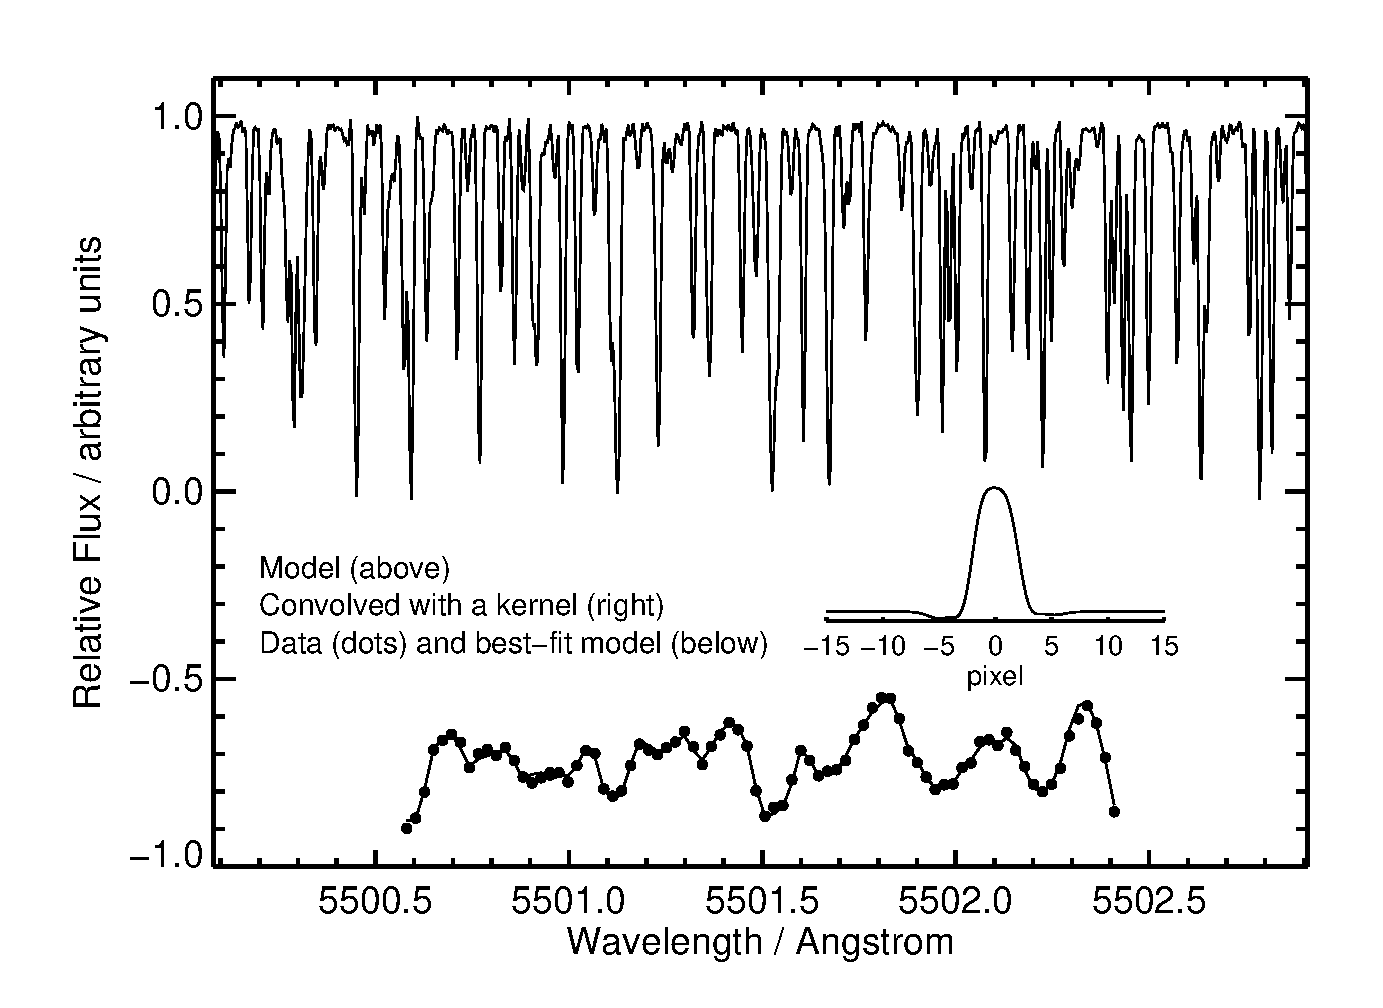
\includegraphics[scale=0.45]{het/convolution_kernel.eps}
\caption{Illustration of convolving the iodine atlas (sharp solid
  lines) with a kernel (middle right insert) to fit the observed
  iodine lines (black dots near the bottom, with best-fit model
  plotted in solid line).
\label{het:fig:convkernel}}
\end{figure}
%----------------------------------------------------------------


How well the IP is being modeled can be tested by fitting a pure
iodine spectrum taken by the spectrograph
(Figure~\ref{het:fig:convkernel}), with the continuum source being
either a lamp or a (mostly) line-free B star. Such spectra are often
referred to as the iodine spectra (or frames or flats), or the B star
iodine spectra. The typical $\chi_\nu^2$ value that we obtain for
fitting \het\ iodine spectra with a generic IP model (Gauss-Hermite
polynomials) is about 2-5, while for Keck/HIRES, the \chisq\ value is
typically around 1 (Figure~\ref{het:fig:iodchunkcomp}). The origin of
this difference in \chisq\ does not seem to rise from a
signal-to-noise difference in the spectra
(Figure~\ref{het:fig:checksnr}).


%----------------------------------------------------------------
% Comparison between HET and Keck chunk fit
% plot made by ~/Exo.../HET.../plots_general/fit_demo/plotfit.pro
\begin{figure}
\centering
\subfloat[\het\ Chunk]{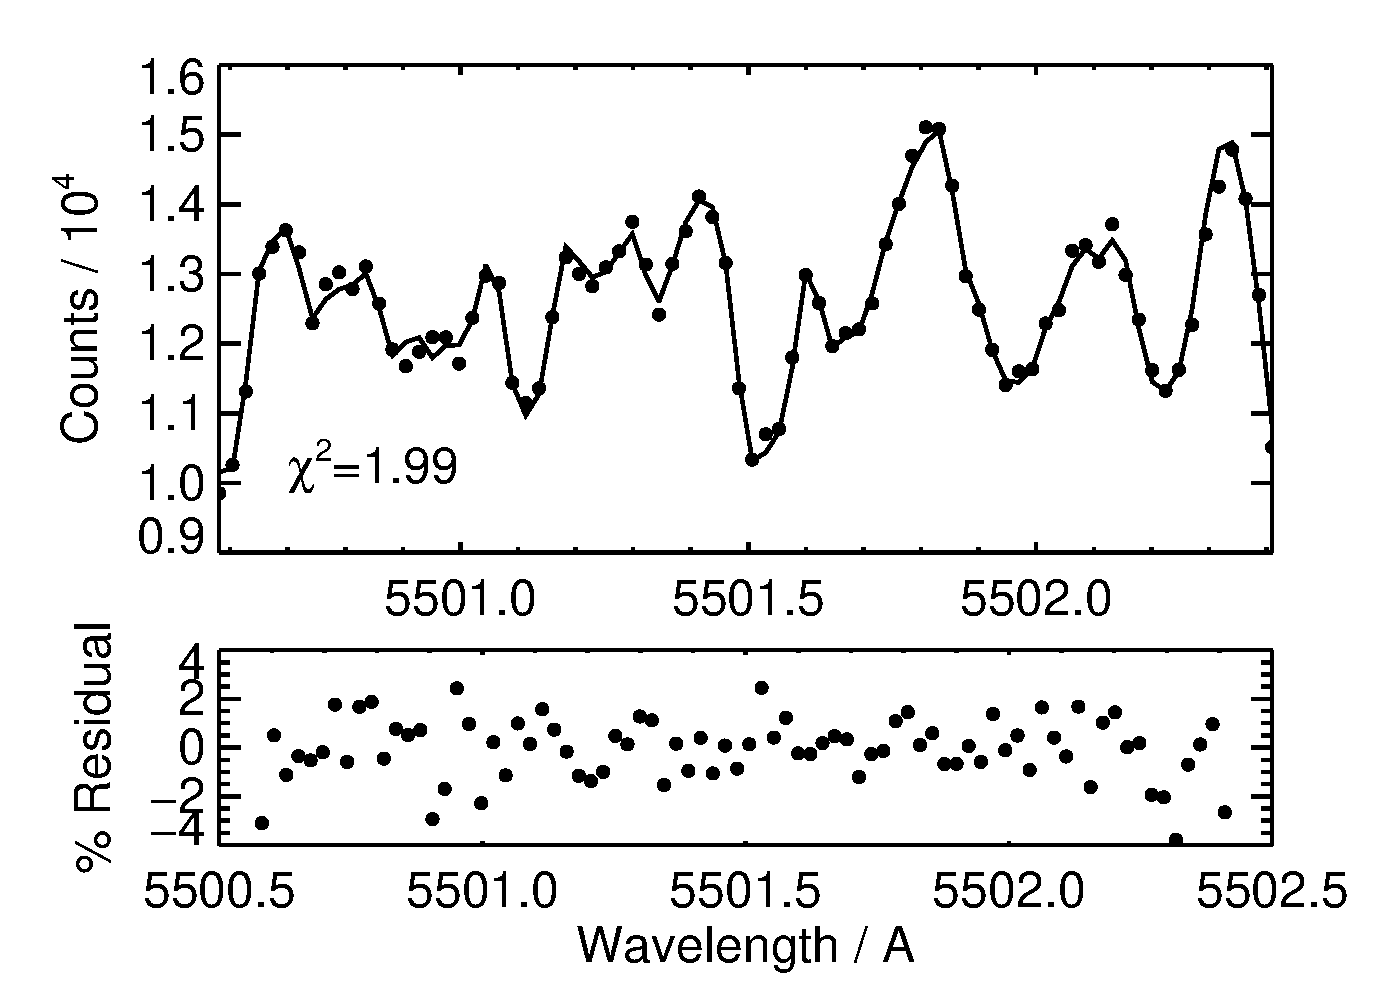
\includegraphics[scale=0.35]{het/20120124.176005.chunk189.eps}}
\subfloat[\keck\ Chunk]{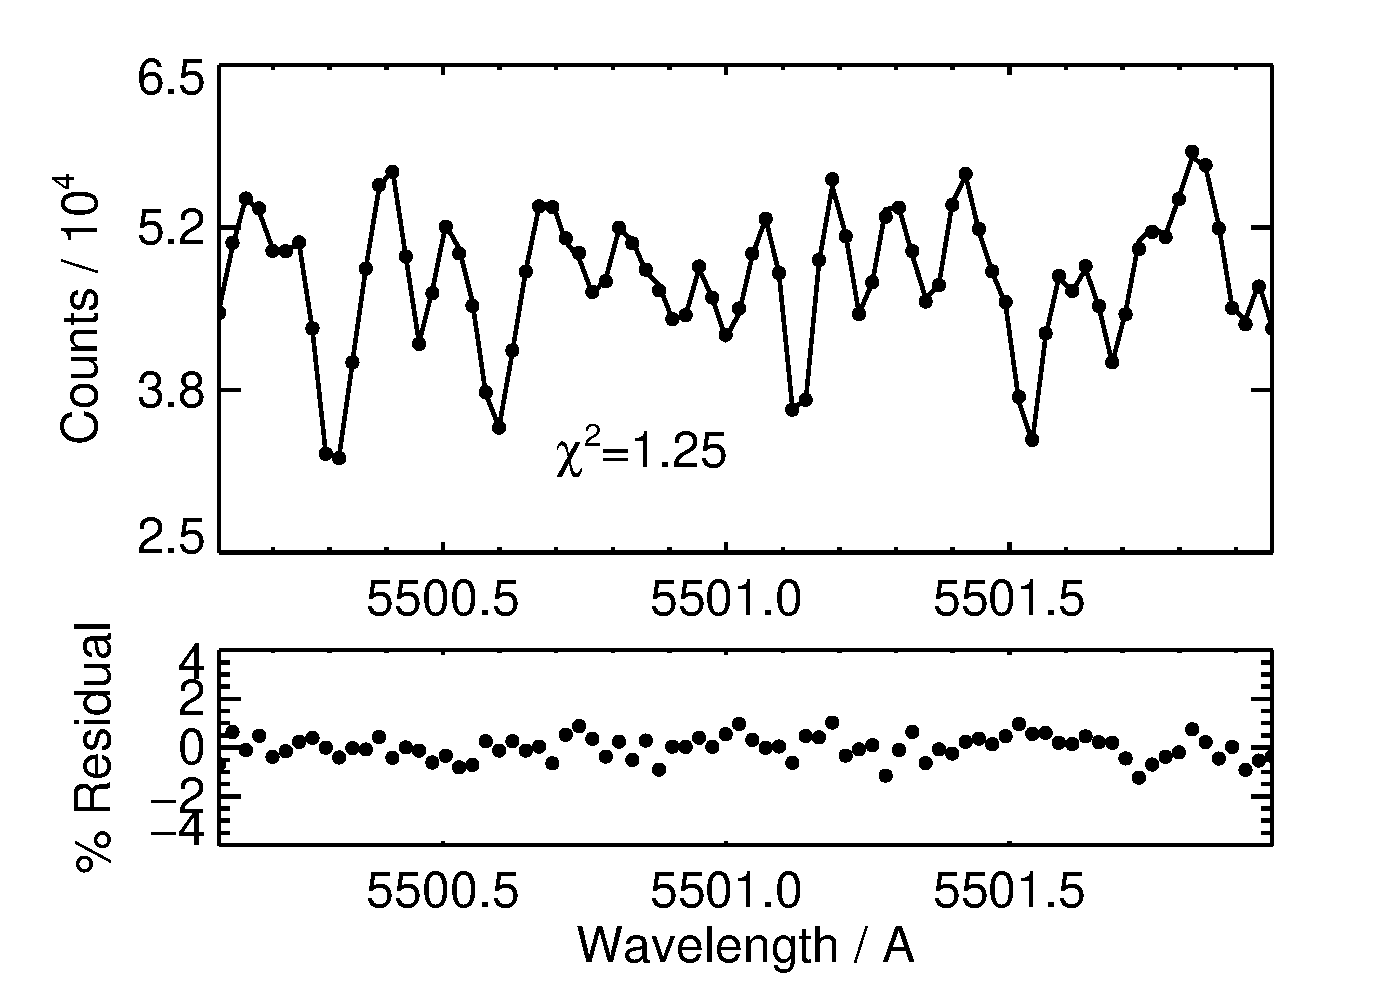
\includegraphics[scale=0.35]{het/rj82.77.chunk308.eps}}
\caption{Comparison between fits for a typical iodine-only chunk using
  \het\ data (left panel) and \keck\ data (right panel). Bottom panels
  are showing the residuals against best-fit models, plotted on the
  same $y$-axis scale. \het\ fit is significantly worse than \keck,
  which we believe is one of the major drivers behind \het's poorer RV
  precision. 
\label{het:fig:iodchunkcomp}}
\end{figure}
%----------------------------------------------------------------



%----------------------------------------------------------------
% HET and Keck chunk SNR and fit comparison
% plot made by
% ~/ExoPlanet-2010-2011/HET-HRS-IP/05-Iodine_FTS_investigation/check_snr.pro and saved in ./plots/a
\begin{figure}
\centering
\subfloat{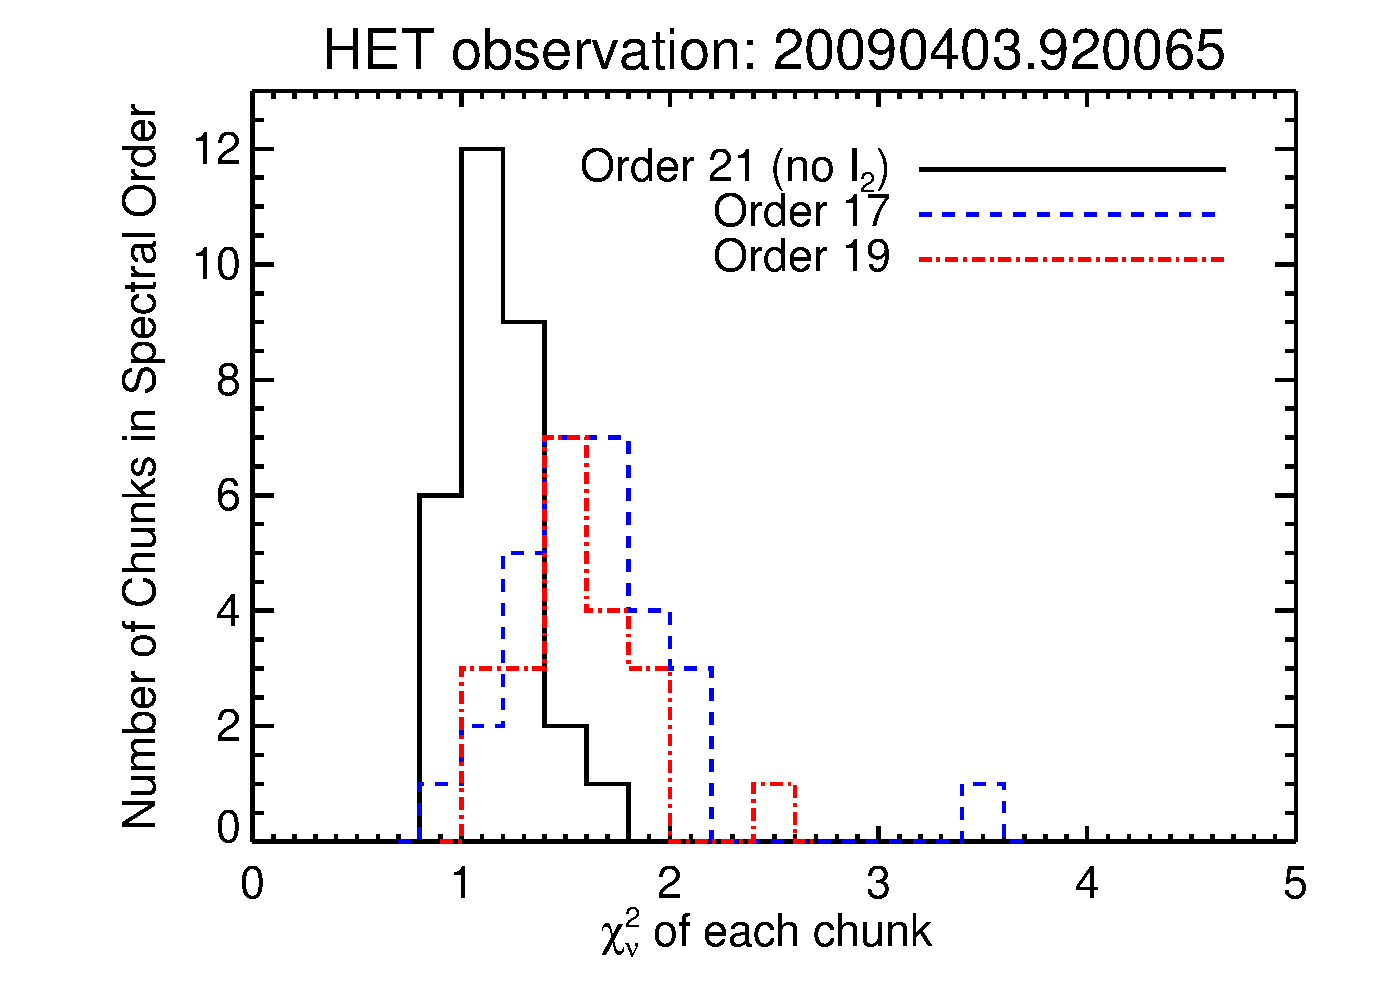
\includegraphics[scale=0.3]{het/het_check_snr.eps}}
\subfloat{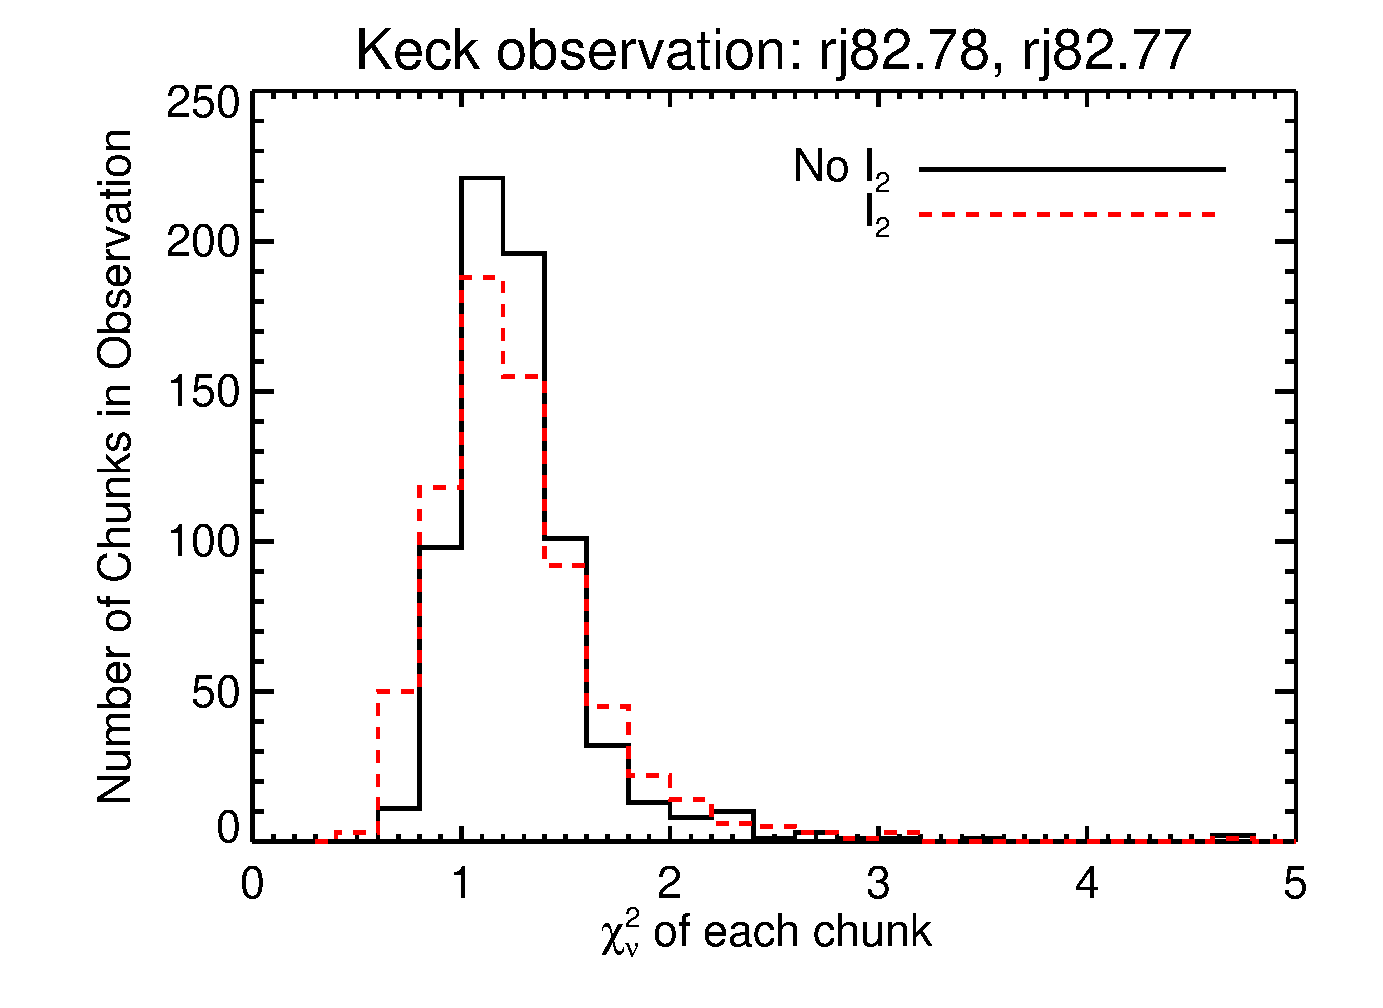
\includegraphics[scale=0.3]{het/keck_check_snr.eps}}
\caption{Comparison of fits for iodine-free region/observation
  (fitting a straight line for each chunk) and for iodine
  region/chunks. The left panel is for \het\ data in one observation,
  but using spectral orders with or without iodine lines. The right
  panel is for \keck\ data in two different observations with and
  without iodine cell in place. The fits for iodine-free spectral
  chunks turn out to be consistent what is expected with photon noise
  for both \het\ and \keck. This eliminates additional noise as a
  suspect in contributing to the bad fits to \het\ iodine spectra.
\label{het:fig:checksnr}}
\end{figure}
%----------------------------------------------------------------



The current ``go-to'' IP model for \hrs\ is the very versatile,
orthogonal, 11-parameter Gauss-Hermite polynomial (GH), which was
described in Chapter~\ref{chap:doppler}. Another customized IP for
\het\ was tried out by CPS using the sum of Gaussians, the same as
the one used for \keck\ but having the wings at different locations
with different default widths. The two IPs basically perform at a
similar level, with GH being slightly better
(Figure~\ref{het:fig:ghgau}). We have also tried several other
functional forms such as GH convolved with a top hat function with a
varying or fixed width, Lorentzian-Hermite (replacing the Gaussian in
GH with a Lorentzian), which all performed marginally worse than GH,
just like the sum of Gaussians. Or, more precisely, these IPs all seem
to be ``equally bad''.


%----------------------------------------------------------------
% Comparing 2005 and 2008 data, with GH and Gaussian IPs
% plot from ~/ExoPlanet-2010-2011/Professional_Development/201000-NSF_Jason/plots/
\begin{figure}
\centering
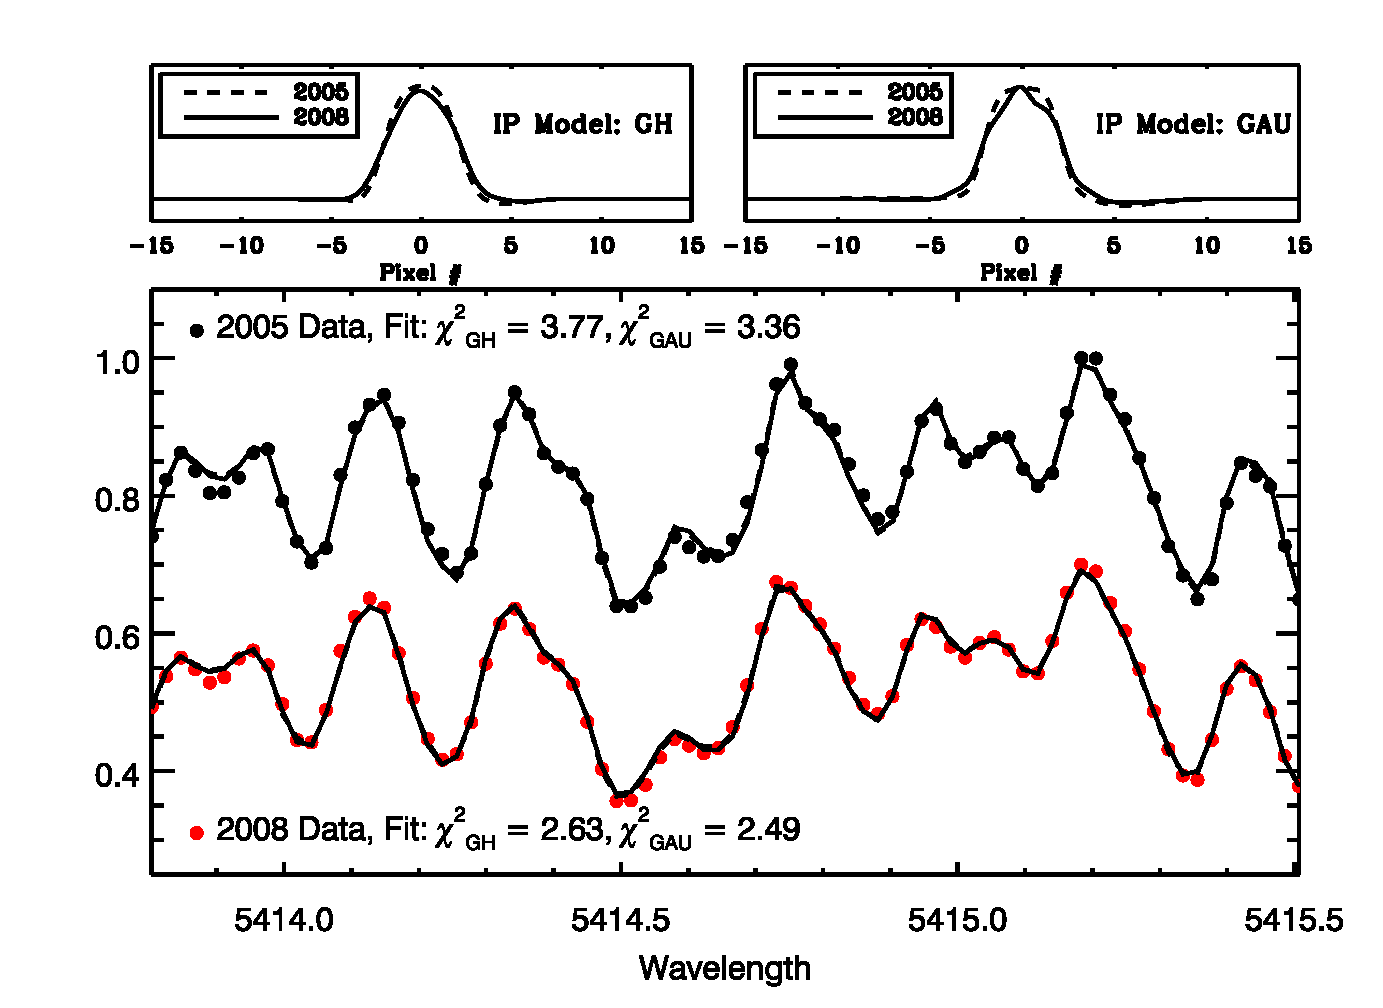
\includegraphics[scale=0.45]{het/iodfit.eps}
\caption{Illustration of fitting the iodine-only data (bottom panel)
  using different IPs (top panels), in this case, using GH and sum of
  Gaussians (GAU). These two IPs are practically ``equally bad",
  having similarly large reduced $\chi^2$ but neither produces a
  satisfactory fit. It is also interesting to see how ``stable" the
  best-fit IP can be across the years (i.e., in 2005 vs.~2008) and its
  smoothness, hinting that the best IP may take a simple, slowly-varying form. 
\label{het:fig:ghgau}}
\end{figure}
%----------------------------------------------------------------


We then looked for clues in the Fourier space:
Figure~\ref{het:fig:fftip} plots the Fourier transform power spectrum
of the \het\ data (using the {\it fft} procedure in IDL) for the
entire $\sim$1000\AA\ 1-D extracted spectrum used for precise-RV
purposes; with \keck\ data also plotted for comparison). At high
frequency in Fourier space, or shorter periods in pixel space, i.e.\
on small scales, the power spectrum is dominated by the signature of
the IP. A ``null'' in the power spectrum at 4.3 pixel is clearly
visible, which suggests some sort of sharp feature, and indeed, it
exactly corresponds to the slit width of \het\ projected onto the
detector at a resolution of R $=$ 60,000. This feature is a direct
result of the fact that HRS has the slit in front of a round fiber,
creating somewhat of a sharp feature in its IP, unlike the slit-fed
\keck.


%----------------------------------------------------------------
% Comparing Keck and HET IPs in Fourier space
% plot from screen shot of a slide in
% ~/ExoPlanet-2010-2011/Professional_Development/20150727-ThesisCommMeet/
% original plot is from ~/Exo../HET.../06-line.../powspec.pro and stored in ./plots/
\begin{figure}
\centering
\includegraphics[scale=0.35]{het/fftip.eps}
\caption{Fourier transform or power spectrum of a \het\ iodine-only
  spectrum (black dots) and its smoothed version (blue line). There is
  a clear signature of the \het\ slit at 4.3 pixel (corresponding to
  slit width for resolution R $=$ 60k). For comparison, the red curve
  is for \keck\ data, which shows no clear signature of a slit,
  because \keck\ is not fiber-fed and the PSF of the star falls mostly
  within its slit.
\label{het:fig:fftip}}
\end{figure}
%----------------------------------------------------------------


Upon seeing the Fourier transform of the \het\ data, we tried out
another IP using GH multiplying a triangle (with a half width of 2.4
pixel and a height of 1), whose Fourier transform has a null at 4.3
pixel, and it produced the best fit among all IP models we have
ventured. Figure~\ref{het:fig:iodipcomp} illustrates this new fit in
comparison with the GH IP fit, although it was perhaps
still equally bad. At this point, we have already suspected that
the ``ground truth'' for the iodine lines, the iodine atlas, which was
created from an FTS scan, may be problematic. It would not be possible
to derive a correct form for the IP using a wrong iodine atlas, and
thus we shift our priority towards validating the iodine cell FTS and
investigating possible changes in the cell, which is described in the
next section.


%----------------------------------------------------------------
% Comparing fits with two IPs: GH, and GH+triangle
% plot made by ~/Exo.../HET.../plots_general/fit_demo/compfit.pro
\begin{figure}
\centering
\subfloat{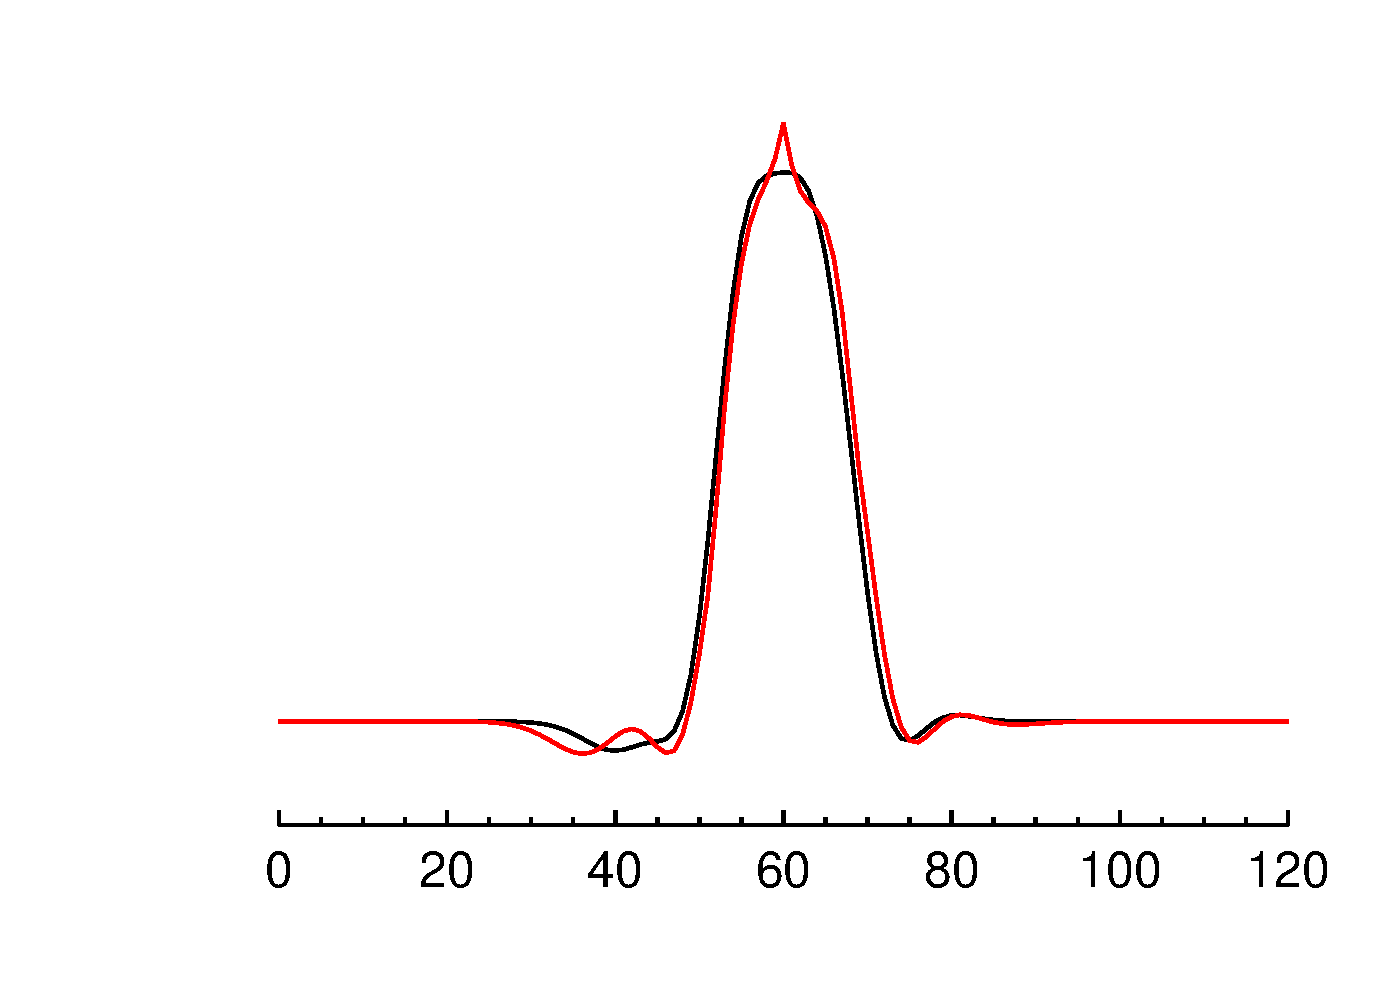
\includegraphics[scale=0.3]{het/20120124.176005.chunk191.compip.eps}}
\subfloat{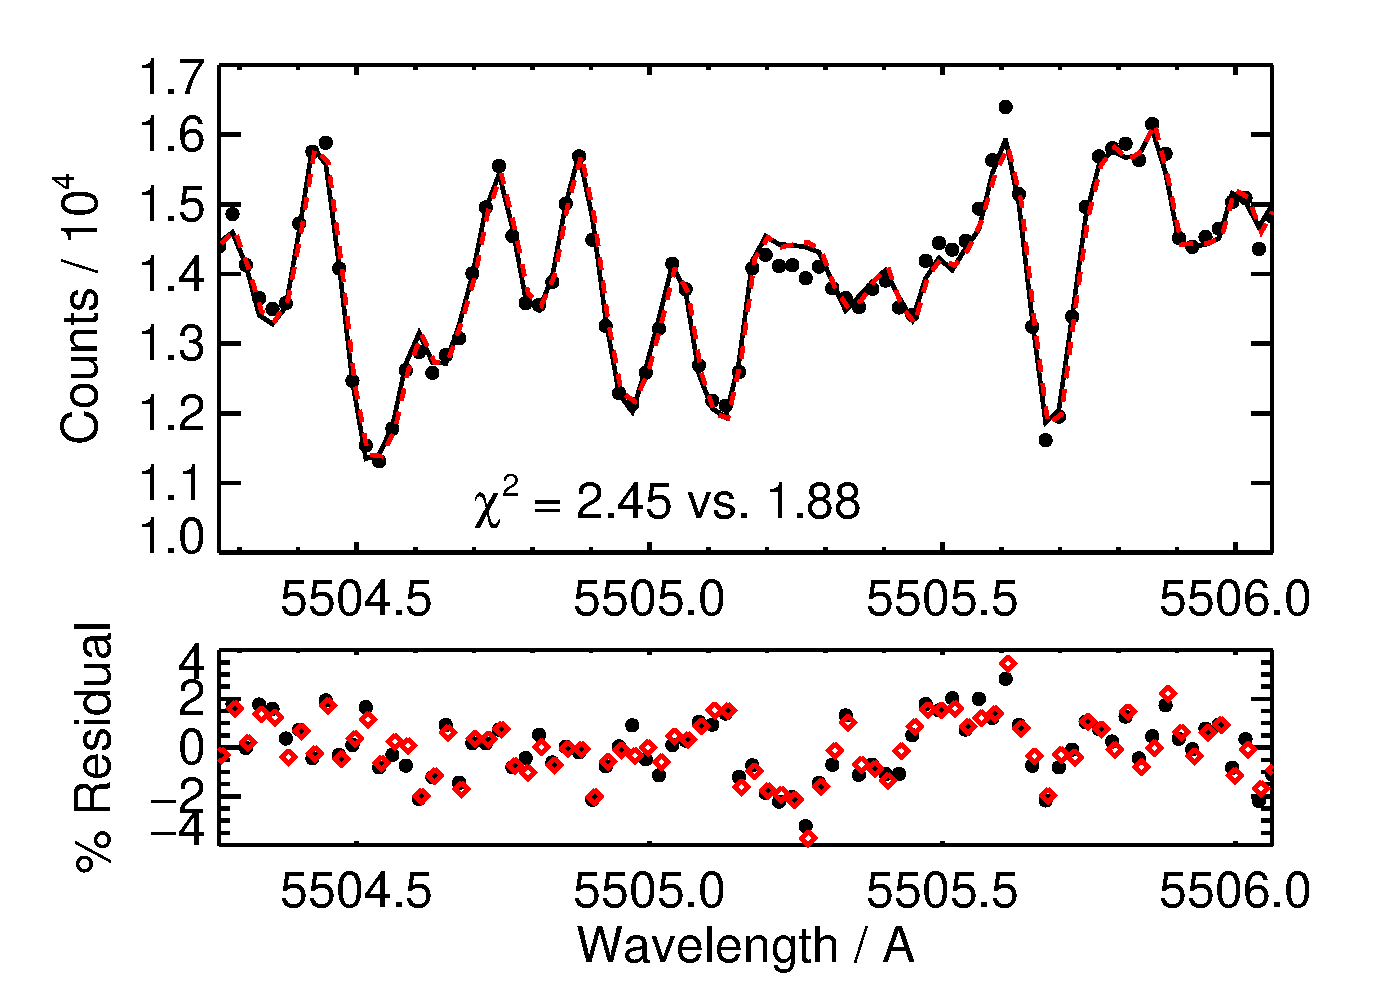
\includegraphics[scale=0.35]{het/20120124.176005.chunk191.compfit.eps}}
\caption{Introducing a sharp feature into the \het\ IP model, a
  triangle on top of the GH IP (red curve in the left panel), produces
  a better fit, somewhat to our surprise. The black in the left panel
  is the best-fit GH IP. GH$+$triangle is the IP model that produces
  the least $\chi^2_\nu$ among all of our IP models. However, as shown
  by the right panel, the two fits barely have any visible difference
  (red curve for GH$+$triangle IP and black for GH; bottom panel plots
  the residuals). Such a sharp feature in the IP is nonphysical, and we
  interpret this results as a hint for an unreliable iodine atlas
  (the sharp peak at the center is perhaps the IP model trying to
  ``stretch" the iodine lines deeper; see Section~\ref{het:sec:fts}
  for more details).
\label{het:fig:iodipcomp}}
\end{figure}
%----------------------------------------------------------------


Besides the problem with the iodine atlas, which fundamentally
prevents us from finding a precise IP, we know for sure that the GH
function does not work very well. We have two lines of evidence
supporting this statement. The first one is that the GH IP performs
terribly on \keck\ data because the L-M least-\chisq\ fitter has
trouble converging (unless fine-tuned and informed from previous fits
using sum of Gaussians; \citealt{2013AAS...22114908V}). The second
piece of evidence is that we tried to fit GH to unsaturated ThAr lines
in \het\ calibration frames, and it often fails to converge onto a
good fit to the ThAr line. 

To end this section with a somewhat positive note, we present a
promising lead for a better IP function for \hrs, the modified Moffat
function:
\begin{equation}
[1+(x/\theta)^2]^{-\beta\cdot(x/\delta)^2}
\end{equation} 
It is called the ``modified" Moffat function because the original
Moffat function does not have the $(x/\delta)^2$ term. We added this
term to add flexibility at the wings to enable change of
characteristic IP width while preserving wing
profile. Figure~\ref{het:fig:moffat} illustrates the results using the
modified Moffat fitting a ThAr line (insert), and also the
$\chi^2_\nu$ distribution of all spectral chunks for this new IP
compared with the GH IP. Unfortunately, the modified Moffat function
does not always fit a ThAr line (starting with uninformed initial
guesses), so it faces the same problem as GH. However, it only has
four parameters and they are mostly physically meaningful. For
example, one can imagine that the $\theta$ parameter describes some
characteristic width. This makes this function easier to work with than
GH.

One can image getting a better fit by adding small perturbation terms
to the modified Moffat IP to account for asymmetries and subtle wings
due to scattered light. Moreover, the modified Moffat function is
potentially applicable to other fiber-fed instruments, since such
instruments are likely to have IPs with the same characteristic flat
top and sharp wings. We hope to continue this effort after the iodine
atlas problem is resolved (see next section) and carry on this
knowledge to other projects such as the new HRS and MINERVA
(Chapter~\ref{chap:conclusion}).


%----------------------------------------------------------------
% Fitting with a Moffat function
% plot made by ~/ExoPlanet-2010-2011/HET-HRS-IP/06-line_through_dots/thar.pro
% and stored in ./plots/
\begin{figure}
\centering
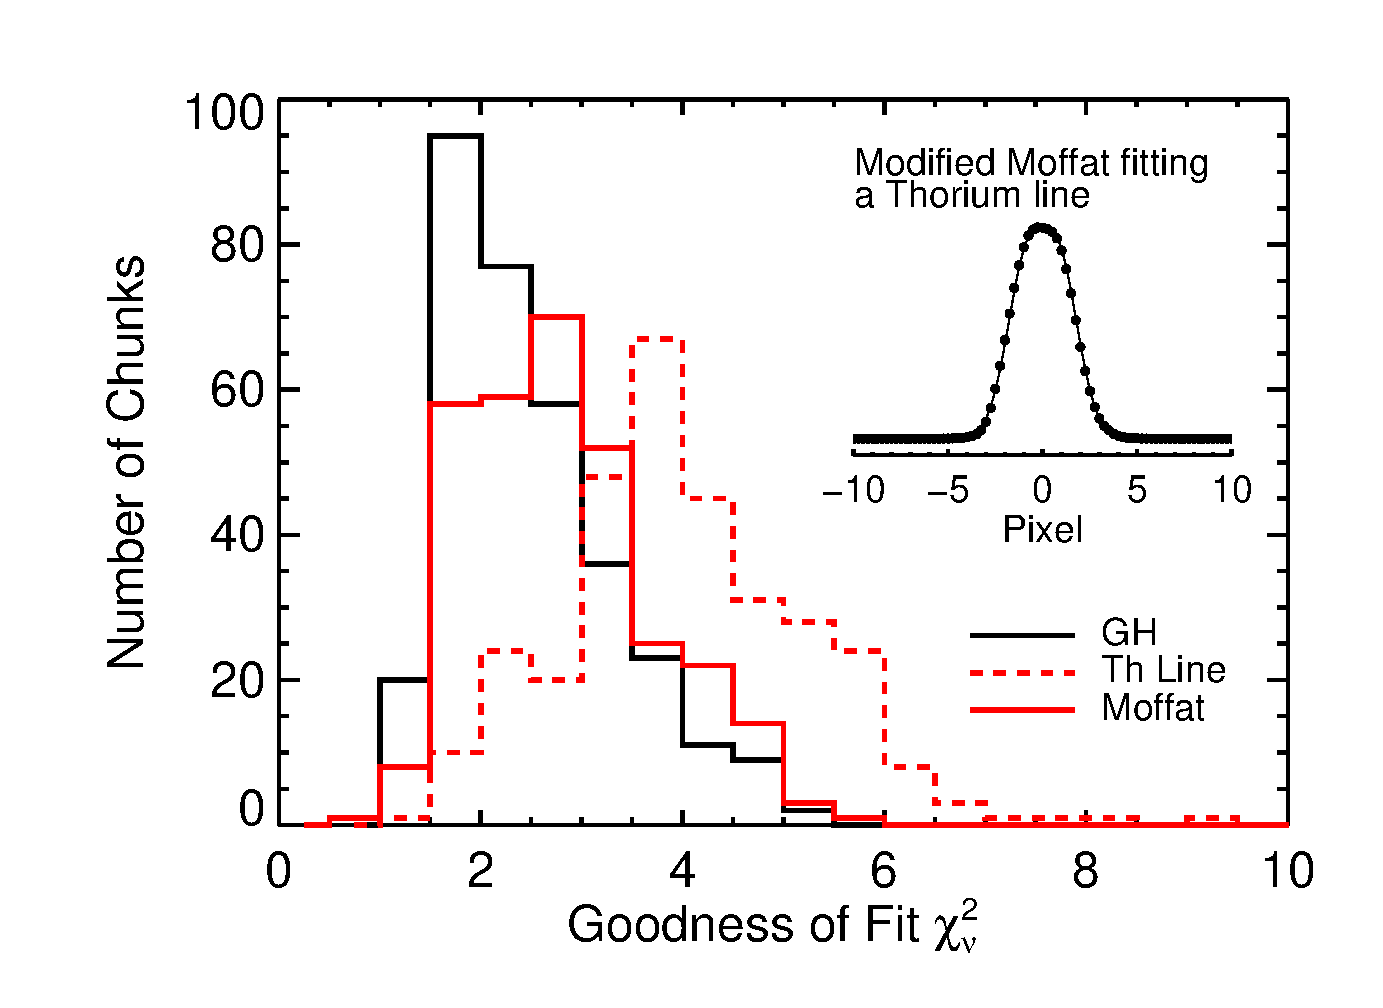
\includegraphics[scale=0.45]{het/thar_vs_moffat.eps}
\caption{Histogram of goodness of fit, $\chi^2_\nu$, values for
  spectral chunks of an iodine spectrum. The modified Moffat function
  (red) performs almost equally well while having only 3 parameters,
  com- pared with the complicated 11-parameter GH function (black
  solid). Red dashed histogram is for fits using a ThAr line profile
  as IP. The insert is showing the modified Moffat function can fit a
  ThAr line quite well.
\label{het:fig:moffat}}
\end{figure}
%----------------------------------------------------------------





%%%%%%%%%%%%%%%%%%%%%%%%%%%%%%%%%%%%%%%%%%%%%%%%%%%%%%%%%%%%%%%%%%%%%%%%%%%%%%
\section{Investigation on the Fourier Transform Spectrometer Scans of the Iodine Cell}\label{het:sec:fts}

% HET FTS

As discussed in the previous section, successful modeling of the
iodine observations (B star spectra taken through the Iodien cell) is
a good indication of a working radial velocity (RV) pipeline. At
Keck/HIRES, which has demosntrated 1 m/s RV precision over the years,
the modeling of the iodine observations yields a reduced chi-square
(\chisq) value of typically 1.05. However, for HET/HRS iodine
observations, with the same RV pipeline used at Keck, the typical
\chisq\ value is $>2$ or even $>5$ for some observations. 

We have explored one of the two model components for modeling iodine
observations, the choice of IP. In this section, we examine the other
model component, the iodine atlas, that is, the ``ground truth''
spectrum for the iodine absorption lines unique to the \het\ iodine
cell. A ``ground truth" iodine atlas is crucial for the precise iodine
radial velocimetry. It is used for modeling the observed iodine lines
in the stellar$+$iodine RV observation to anchor the absolute
wavelengths and the spectrograph response function. 


%%%%%%%%%%%%%%%%%%%%%%%%%%%%%%%%%%%%%%%%%%%%%%%%%%%%%%%%%%%%%%%%%%%%%%%%%%%%%%
\subsection{Why did we suspect the iodine atlas?}

As we were investigating the reasons behind the apparent `bad fit' of
\het\ iodine observations, we decided to check the quality of the
existing iodine atlas. An iodine atlas is normally obtained using a
Fourier Transform Spectrometer (FTS; whose mechanism is just like a
Michelson interferometer). The scan and its subsequent data reduction
provides very high resolution spectrum (translated from Fourier space
into real space) with typically $R > 200,000$-500,000.\footnote{It is worth
noting here that although FTS normally provides wavelength solutions
(from the registered arm lengths), but because of the inaccuracy of
the default reported wavelengths, the final wavelength solution for
the iodine atlas is usually derived from a theoretically computed iodine
line list (e.g., \citealt{iodinespec5}).}

The existing iodine atlas for the \het\ cell is from an FTS scan taken
at the National Solar Observatory at KPNO using the Babar FTS
(nicknamed for its large size; this machine has been decommissioned)
in 1993. The main reason is that the FTS scan was taken almost two
decades ago, and during this time the cell may have gone through
changes (such as temperature, leaking or condensation, etc., though
unlikely, since the cell was designed to be stable). This would mean
that the FTS scan is out of date and inaccurate, and it could explain
the `bad fits' to the iodine observation.

We therefore took the HET/HRS cell to the National Institute of
Standards and Technology (NIST) and obtained a new FTS scan in 2011
(an effort carried out by Jason Wright, Ming Zhao, Stephen Redman and
others at NIST; data reduction done by Stephen Redman). A close
comparison between this new scan from NIST and the old scan at KPNO
reveals that they have many differences:
\begin{itemize}
  \item The overall line depths are very different --- the NIST scan
    has deeper lines.
  \item The absolute wavelength solutions are different, and the
    drifting of wavelength solution or the dispersion scales at
    different wavelength are also different.
  \item Even after we adjust the `normalization' level of the NIST
    scan (assuming the FTS data has normalization issues or low
    frequency noise/offset), the line ratios of the two scans still
    exhibits differences.
\end{itemize}

Figure~\ref{fig:fts_old_new} shows the comparison between the two
scans in a selected 2\AA\ region. As the two scans also differ in
resolution (the NIST scan has a higher resolution), the middle panel
is a more direct comparison: the NIST scan has been convolved down to
the same resolution with the KPNO scan; it is also shifted in
wavelength space so that the two scans match in absolute wavelength
solution; and it is adjusted to a different ``normalization'' level to
match with the KPNO scan as much as possible in order to compare their
relative line ratios.

    
%----------------------------------------------------------------
% Figure: HET FTS, KPNO old scan vs. NIST new scan
\begin{figure}[!th]
\centering
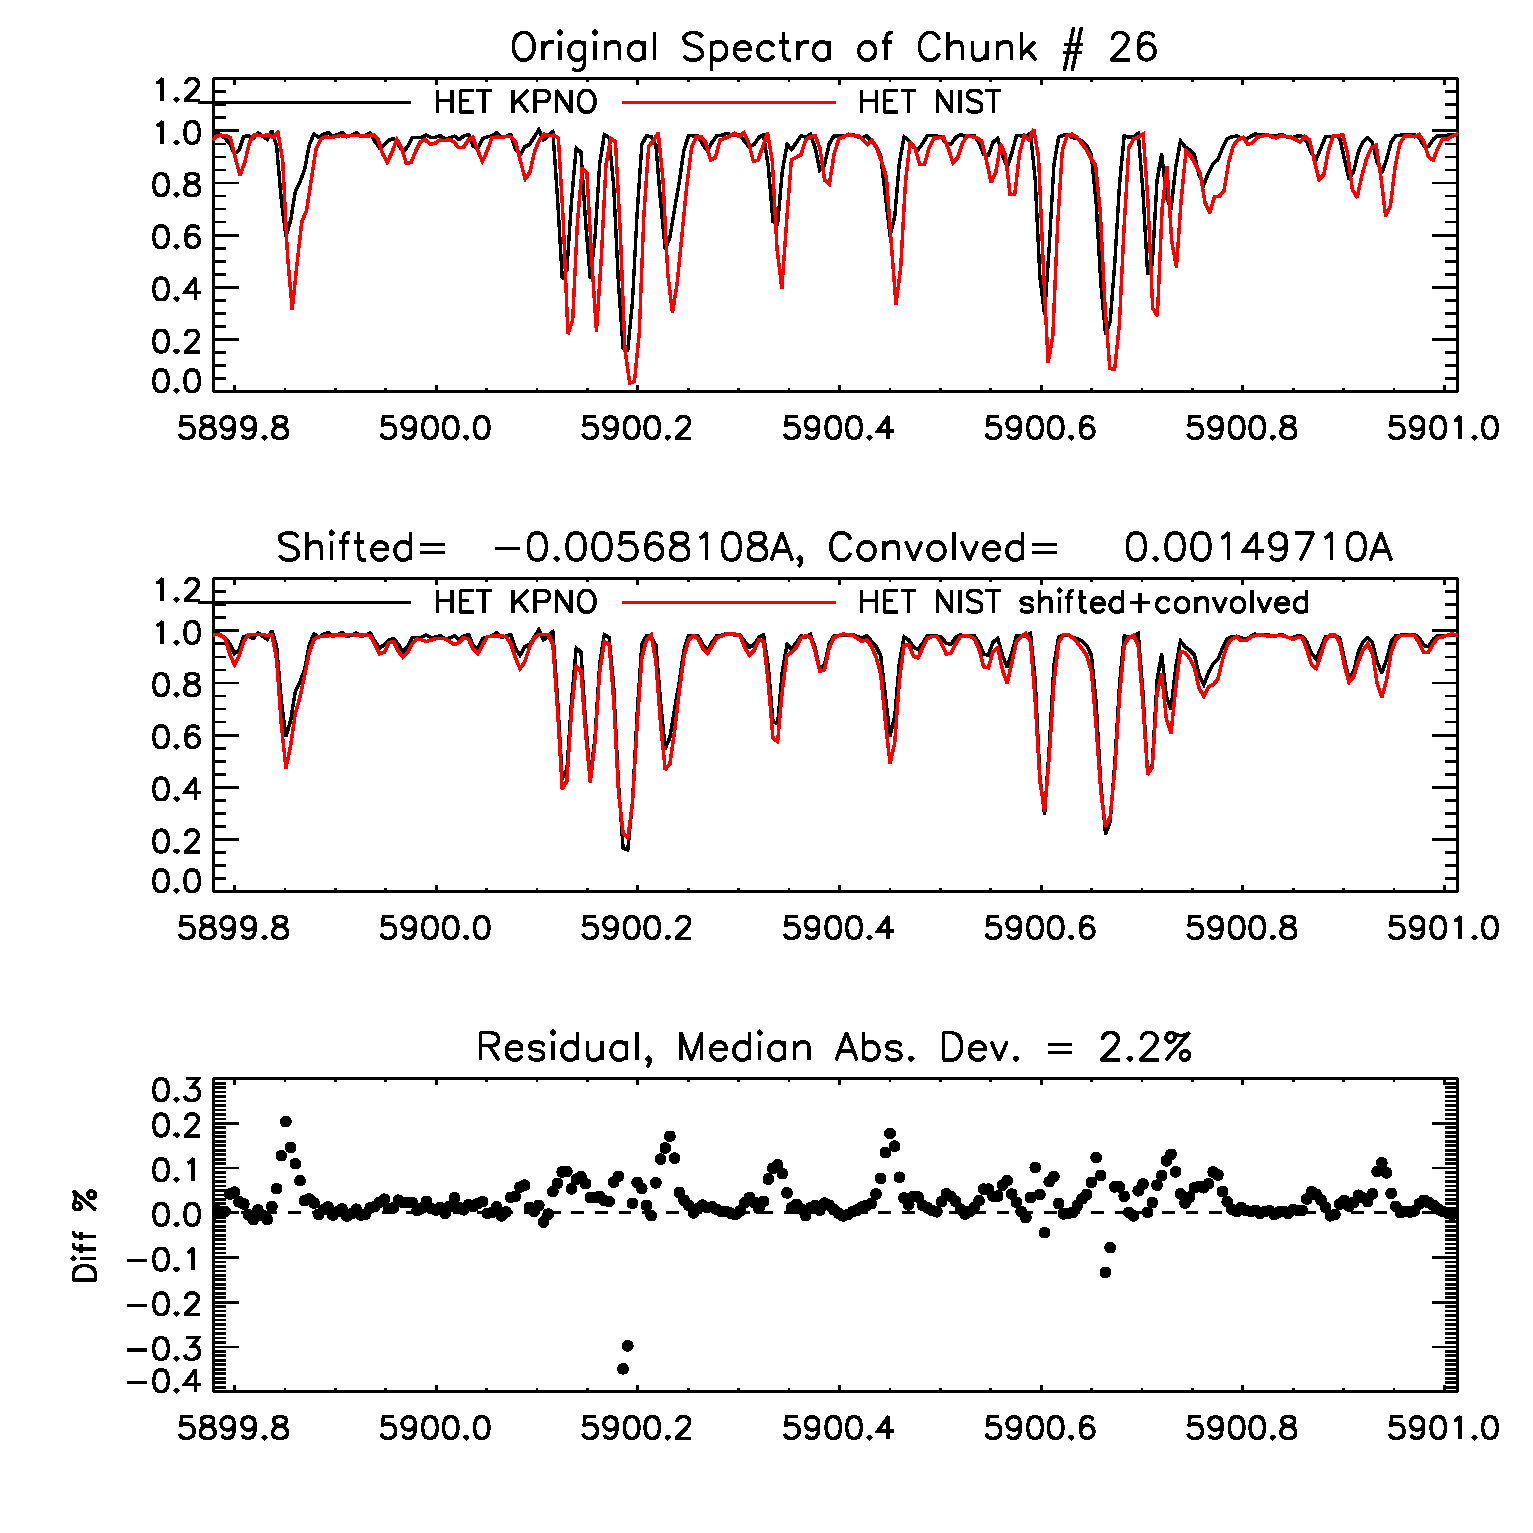
\includegraphics[angle=0.,scale=0.45]{het/compare_het_fts_26.eps}
\caption{Comparison of the KPNO FTS scan (black) and the NIST FTS scan
  (red) for the HET/HRS iodine cell for a selected
  1.5\AA\ chunk. \textbf{Top:} Two scans at their native resolution
  and original wavelength solution. \textbf{Middle:} Comparison of the
  two scans after adjusting the normalization, shifting, and
  convolution for the NIST scan to match the KPNO scan for a more
  direct comparison of line depths/ratios. \textbf{Bottom:} Residuals
  of the middle panel, NIST spectrum minus the KPNO spectrum. The
  median absolute deviation between the two spectra is 0.02
  (2\%), though at many places, especially at line centers, the two
  can differ by up to 5--10\%.
  \label{fig:fts_old_new}}
\end{figure}
%----------------------------------------------------------------

We initially suspected that the NIST scan was problematic. The reason is
illustrated in the left panel of Figure~\ref{fig:chisq_old_new}, where
it shows the histogram of \chisq\ values for fitting an selected iodine
observation using the two scans, respectively. Each \chisq\ value is
for a 2\AA\ chunk in this selected iodine observation. It is clear
that the NIST scan provides worse fits.

%----------------------------------------------------------------
% Figure: chisq of iodine observation fit, KPNO old scan vs. NIST new scan
\begin{figure*}[!th]
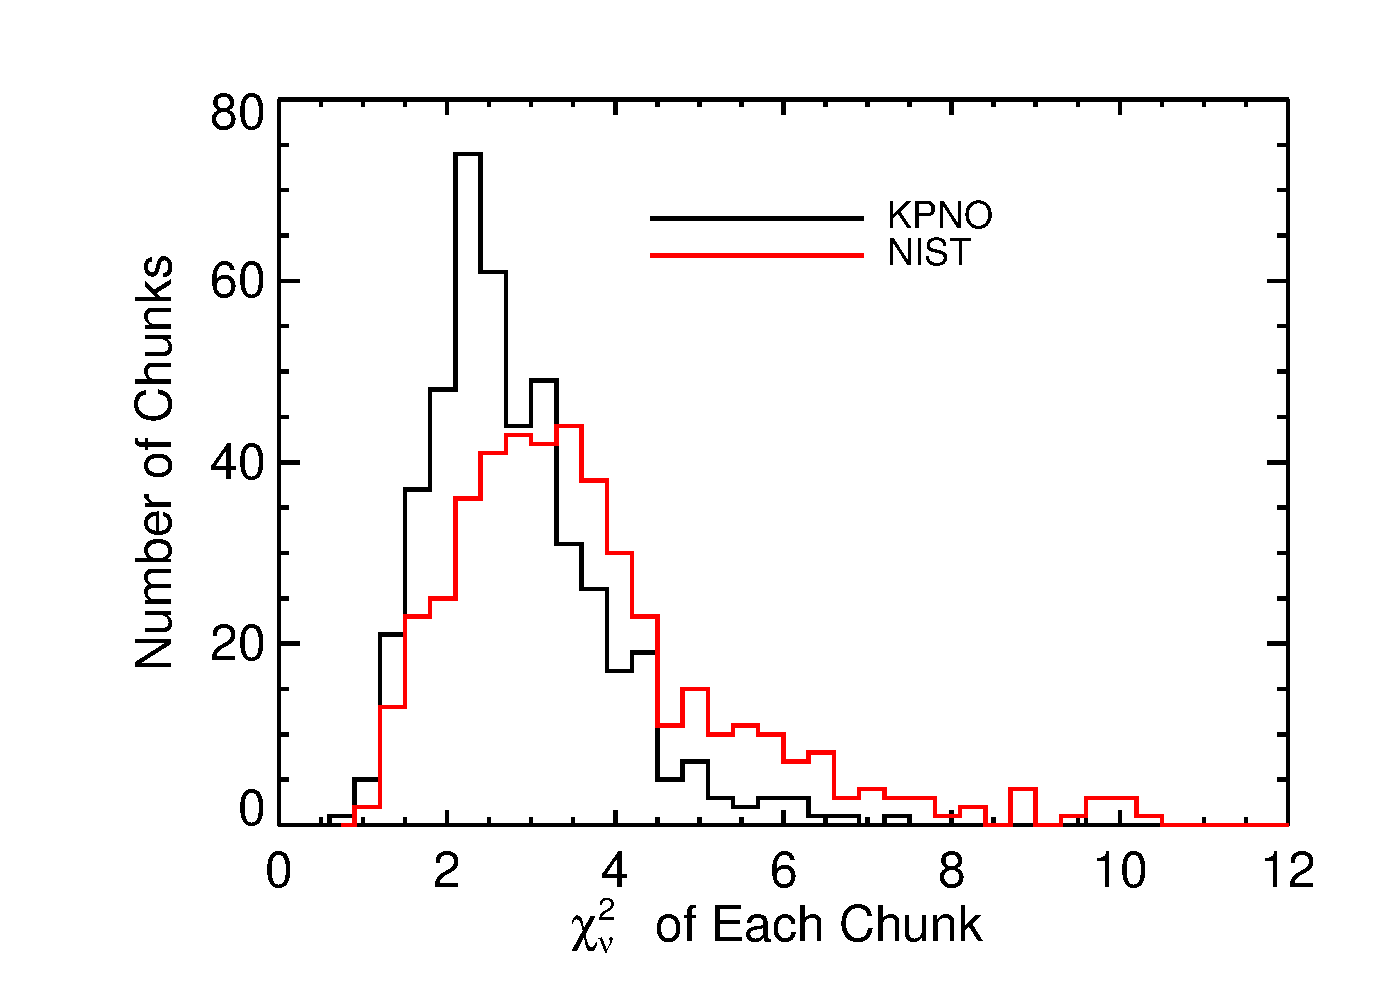
\includegraphics[angle=0.,scale=0.33]{het/hetfts_oldVSnew_chisq.eps}
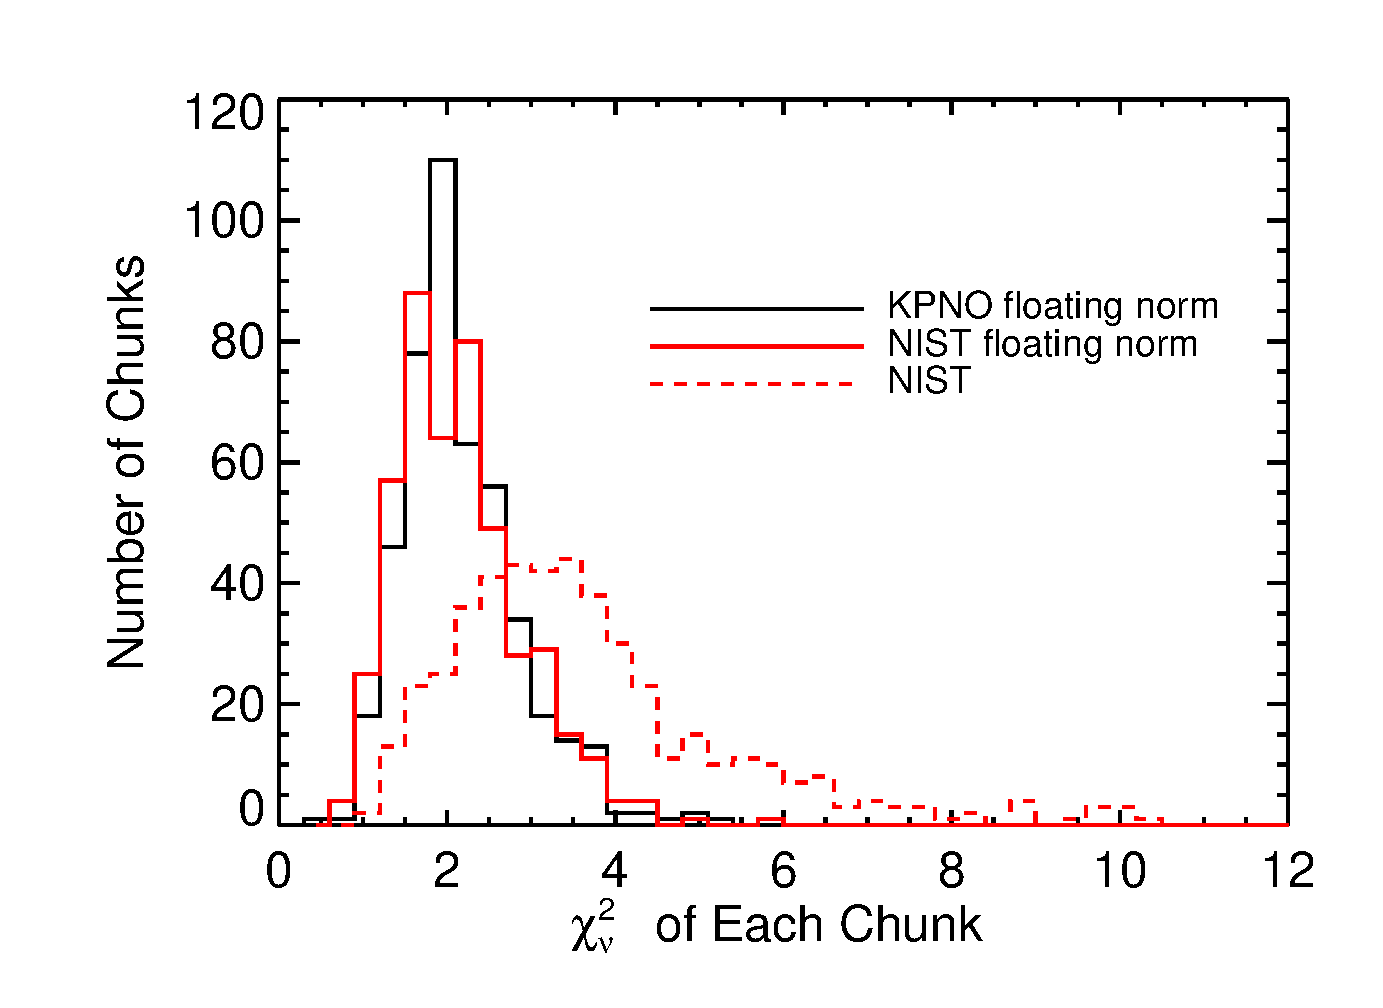
\includegraphics[angle=0.,scale=0.33]{het/hetfts_oldVSnew_chisq_dc.eps}
\caption{Both plots are histograms of \chisq\ values of a single
  iodine observation. Each \chisq\ value in the histogram represents
  the \chisq\ goodness of fit for a $\sim$2\AA\ spectral chunk in this
  iodine observation (each iodine observation is chopped into several
  hundred of chunks and is fitted independently).
%
  \textbf{Left:} \chisq\ histograms for the fit of the iodine
  observation using the KPNO (black) and NIST (red) scan as iodine
  templates, respectively. The KPNO scan obviously performs better.
%
  \textbf{Right:} \chisq\ histograms for the two scans, but both with
  the normalization as a free parameter for each chunk (as we suspect
  the NIST scan has problems in normalization). The two scans now
  perform at essentially the same level. Dashed red line is the same
  red histogram as plotted in the left panel. Notably, the KPNO scan
  also performs better when we float the normalization parameter.
  \label{fig:chisq_old_new}}
\end{figure*}
%----------------------------------------------------------------


Since the direct comparision between the KPNO scan and the NIST scan
has hinted that the `normalization' of the NIST scan might be
problematic, we decide to add a free parameter to account for this
`normalization error' when fitting the iodine observation. The right
panel of Figure~\ref{fig:chisq_old_new} shows the \chisq\ histograms
for the same iodine observation using the two scans, but adding a free
parameter as the `normalization' when fitting each chunk (note: the
normalization parameter is a free parameter for each chunk, not a
global single parameter). The two scans now perform at essentially the
same level.

This is both encouraging and worrisome at the same time. It is
encouraging because it seems that we have found the problem with the
NIST scan, and also have a solution for it. It is very worrisome
because this reveals that:
\begin{itemize}
  \item Even the KPNO cell performs visibly better when we float the
    normalization paramter. This may suggest that there are
    ``normalization'' issues or low frequency errors/noise in the KPNO
    scan as well.
  \item Obtaining high-quality, reliable FTS scans of iodine cell is
    very difficult, and the FTS scans cannot be naively trusted as the
    ``ground truth'' super accurate templates of the complicated iodine
    spectrum.
  \item The reason why adding a ``floating normalization'' fits the
    data better might be because it accounts for optical depths difference
    between the atlas and the actual observations, which may be a result
    of changes in cell temperature or iodine column density in the cell.
  \item The pipeline (when floating normalization as a free parameter)
    cannot distinguish which scan is the ``correct'' one (by \chisq)
    even when two scans differ as much as $\sim$5--10\% at places and
    also have obvious line ratio differneces (see comparison in bottom
    panel of Figure~\ref{fig:fts_old_new}). However, this level of
    difference in FTS may affect the RV precision, and not knowing
    which atlas is the correct one definitely affects our ability to
    search for a better IP and improve the RV precision of \het.
\end{itemize}  

Perhaps even more alarmingly and more puzzling, when we use the KPNO
scan for the iodine cell used at Keck/HIRES to fit an HET/HRS iodine
observation, it yields smaller \chisq\ values than using any of the
other two scans (Figure~\ref{fig:lampi2fit}). The \het\ cell KPNO scan
was taken at the same time using the same FTS machine as the \keck\
cell scan. However, the set-temperatures of these two cells are very
different: the \keck\ cell is designed to work at 50$\degree$C, while
the \het\ cell is designed to work at $70\degree$C. A closer look
reveals that the HET KPNO scan and the Keck KPNO scan have very
similar line depth, with Keck having slightly deeper lines (thus
higher iodine molecule column density).


%----------------------------------------------------------------
% Figure: chisq of iodine observations, NIST vs. KPNO vs. Keck cell 
% plots made by
% ~/ExoPlanet-2010-2011/HET-HRS-IP/05-Iodine_FTS_investigation/compare_fts/compare_fts_fits.pro
% stored in ../plots/
\begin{figure}[!th]
\centering
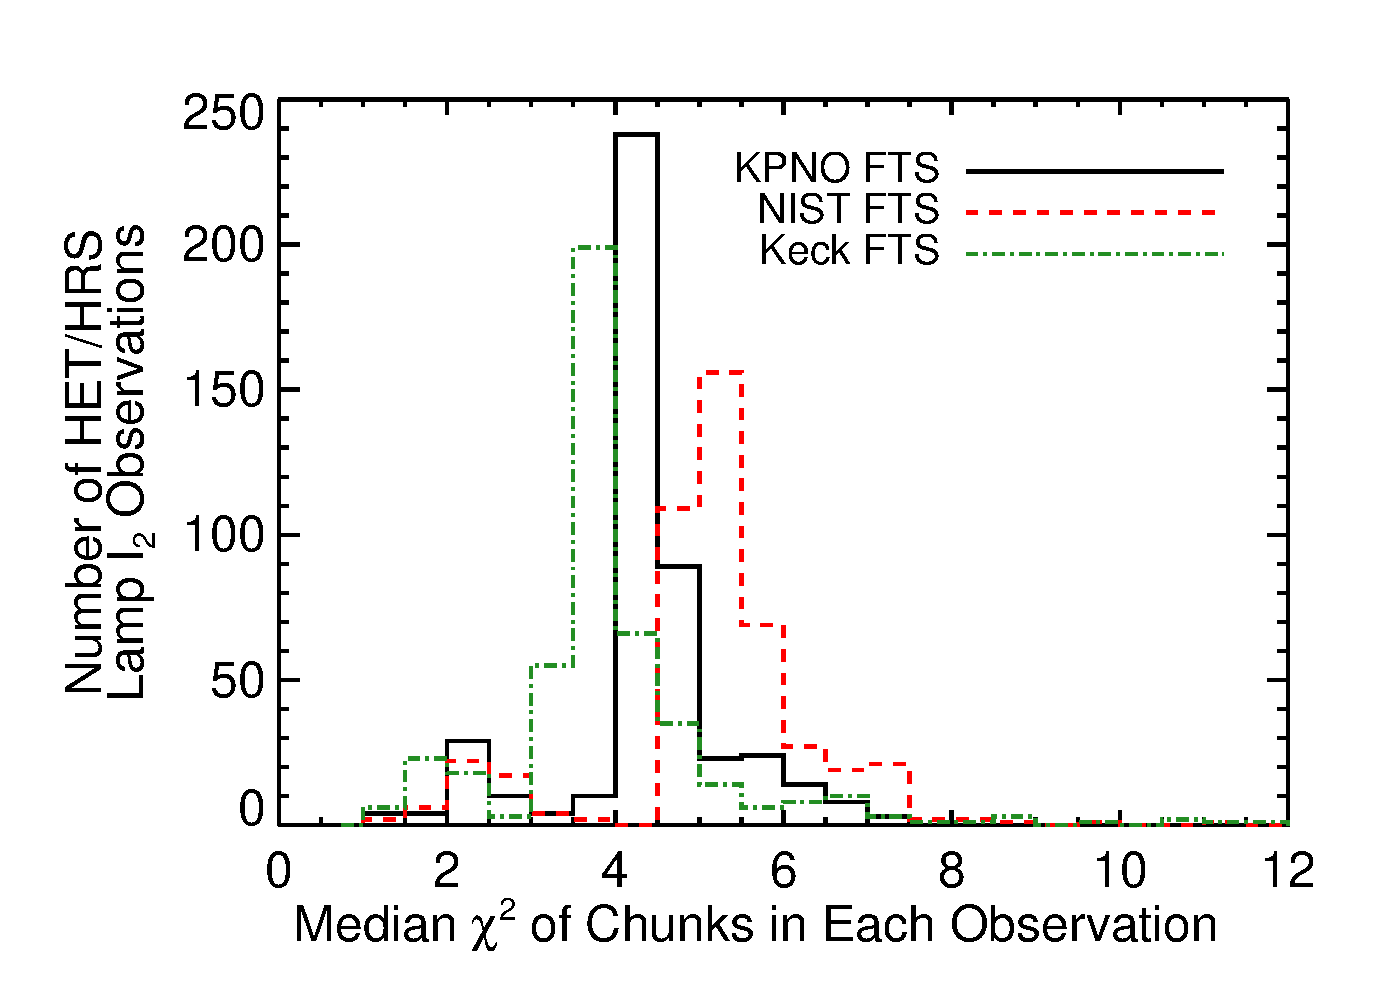
\includegraphics[angle=0.,scale=0.38]{het/het_lamp_i2_fits_kpno_nist_keck.eps}
\caption{Comparison of the median \chisq\ values for fits of iodine
  observations using the \het\ cell KPNO scan (black solid line), the
  NIST scan (red dashed), and the {\em \keck\ cell} KPNO scan (green
  dotted-dashed). Each data point represents the median \chisq\ value
  for all the chunks in a single iodine observation (these are all
  lamp-illuminated -- no B star observation). Results of 550
  \het\ observations are plotted here to illustrate the statistically
  significance. The \keck\ cell KPNO scan provides a better fit than the
  both \het\ scans when fitting \het\ iodine observations.
  \label{fig:lampi2fit}}
\end{figure}
%----------------------------------------------------------------

All of the facts above prompted us to seek a relatively
independent way to perform quality checks for any FTS scan --- not
just comparing their relative qualities or performances. One
natural choice is to obtain spectra taken with high-resolution echelle
spectrographs, which are measurements of the iodine spectrum directly
in the ``real wavelength space'' instead of in the ``Fourier space'', and
thus they serve as good reference spectra as they suffer from
different types of error compared to FTS. Since FTS scans are usually
at a very high spectral resolution ($200,000$--$500,000$), this limits
our choice to essentially only one spectrograph --- the TS12 setting
of the Tull Spectrograph at the 2.7m Telescope at McDonald.

Our goal is to answer the question of {\bf which FTS scan better describes
the \het\ iodine cell: the KPNO one, or the NIST one? Why?} While adding an
additional normalization parameter can provide better fits for the
iodine frames, we cannot afford to add such an additional parameter
when extracting RVs from star$+$iodine data -- this normalization
parameter is highly degenerate with Doppler shift and wavelength
solution parameters, and it will undoubtedly decrease the RV
precision. Another key question is {\bf why the FTS scan for the \keck\
cell works the best.}


%%%%%%%%%%%%%%%%%%%%%%%%%%%%%%%%%%%%%%%%%%%%%%%%%%%%%%%%%%%%%%%%%%%%%%%%%%%%%%%%%%%%%%%%%%%%%%%%%%%%
\subsection{Ultra-High Resolution Echelle Spectra of Iodine Cells}

To break the tie between various FTS scans, we used the TS12 setting
of the Tull Spectrograph at the 2.7m Telescope at McDonald
Observatory, which provided a resolution of 500,000 (based on ThAr
line measurements done by David Doss at McDonald). 

We had two rounds of TS12 runs, both during day time and when the
telescope was scheduled to on Cassegrain instrument and the Tull
Spectrograph room was free for use. For the first run (from September
7 to September 9, 2013; done by Ming Zhao and the author) we measured
the iodine absorption spectrum for the iodine cell at the Sandiford
(2.1m) Telescope, because the HET/HRS cell was still under active use
when we did this test. The main purpose of the first run was to
validate the quality of the TS12 spectrum and whether we can use it to
across-validate the FTS scans. The Sandiford cell also has an KPNO FTS
scan which was taken together with the KPNO scan of the HET cell in
1993, so it also serves the purpose of testing the overall quality of
the KPNO scans.

In the second TS12 run, we measured the spectrum for the \het\ iodine
cell in its new enclosure and temperature controller (along with the
MINERVA iodine cell and the iodine cell on McDonald Harlan J.\ Smith
2.7m telescope; from October 13 through October 16, 2014; carried out
by Ming Zhao, Kim Star, and Joey Schmitt). Our TS12 runs are enabled
by Anita Cochran, Bill Cochran, Phillip MacQueen, and the astronomers
who used the Cassegrain instruments at night (VIRUS-W for the first
run and IGRINS for the second), with great help and excellent
engineering support from David Doss and Coyne Gibson at McDonald
Observatory.

The hardware settings and data reduction methods are the same for both
runs, which are described below.

\textbf{\textit{Hardware Settings:}} We used the TS12 arm of the Tull
Spectrograph, and the specific instrument choices are listed in
Table~\ref{tab:hardware}. Slit \#23 is chosen to maximize SNR while
maintaining sufficient resolution --- it is among the longest slit and
is also the second narrowest slit. The Sandiford cell was kept at a
temperature of 49.9--50.1$^\circ$C, the same as its working
temperature for RV work and its temperature when the KPNO was taken
(50$\degree$C). The \het\ cell was measured at four different
temperatures: room temperature, 50$\degree$C, 60$\degree$C, and
70$\degree$C (its working temperature). 

%----------------------------------------------------------------
% Table: variability analysis results
\renewcommand{\arraystretch}{1.3} % more row spacing for the table
\begin{deluxetable}{rl}
%\rotate
\tabletypesize{\scriptsize}
\tablewidth{180pt}
\tablecaption{Hardware Settings for TS12 Iodine Spectrum Test\label{tab:hardware}}
\startdata
  \hline
  \multicolumn{2}{c}{Tull Spectrograph, TS12, Coude107} \\
  \hline
  Echelle & E1 \\
  Cross Disperser & c \\
  CCD & TK4, 1024$\times$1056 \\
  On-chip Binning & 1$\times$1 \\
  Slit & \#23 (L$\times$W $=30\arcsec \times 0\arcsec .32$)
\enddata
\end{deluxetable}
%----------------------------------------------------------------


\textbf{\textit{Observation:}} A single exposure frame for the iodine
spectrum covers about 1.9\AA\ (Figure~\ref{het:fig:ts12image}). The
dispersion direction runs vertically along the chip with increasing
wavelength when increasing the $y$-axis pixel. The dispersion scale is
about 0.002\AA\ per pixel ($\sim$7 pixels per resolution element). We
immediately preceded or followed each exposure with a flat fielding
frame. The exposure times for the iodine and flat frames are both 45
seconds (90 seconds for \het\ cell) to achieve a signal-to-noise ratio
(SNR) of 160 per pixel (higher for \het\ cell). Neighboring frames
differ by about 1\AA\ in absolute wavelength. If prominent Solar or
ThAr line was predicted within the wavelength coverage of a frame,
then we also took a Solar or ThAr frame to verify the rough wavelength
solution (the exposure time varied --- typically a couple minutes to
up to 10 minutes). We took dark frames (45s each, about 10 frames) in
the morning at the beginning of each day.

%----------------------------------------------------------------
% TS12 raw image
% plot made by ds9 view on spec0248.fits in
% /Volumes/galileo/rv/TS12/raw/, i.e. 2013 data, save as jpg then
% converted online into eps
\begin{figure}
\centering
\includegraphics[scale=0.35]{het/ts12_image.eps}
\caption{One raw image frame taken using the TS12 setting of Tull
  Spectrograph. It contains about 1.9\AA\ of iodine absorption spectrum. 
\label{het:fig:ts12image}}
\end{figure}
%----------------------------------------------------------------


\textbf{\textit{Reduction:}} We combined and averaged all available
dark frames and created a master dark frame. Then we subtracted the
master dark from all flat and iodine frames. After outlier rejection
(cosmic rays, chip defects, etc.), we modeled the scattered light for
each row of pixels by using the region outside the slit image.  We
stacked 160 neighboring rows and fitted a third order polynomial along
the column, and then interpolated for the amount of scattered light
within the slit image region and subtracted it. Both the flat and
iodine frames have scattered light removed. We then normalized the
flat frames and divided each iodine frame by its associated normalized
flat (for the slit image regions only).

\textbf{\textit{Extraction:}} As the slit does not lie perfectly along
the $x$-axis direction on the chip, we corrected for this by cutting
columns along the dispersion direction and cross-correlating the
columns. Then we interpolated and shifted the columns to create an
aligned image, which we stacked along the $x$-axis direction and
obtained the reduced, extracted spectrum. Each spectrum is then
normalized by dividing the estimated continuum (top 5\% counts). Due
to lower quality of scattered light removal near the edge of the chip,
we discarded the top 80 and bottom 80 rows of pixels. Thus the
extracted spectrum from each frame is about 1.6\AA\ across (instead of
1.9\AA). The reduced frames are then `stitched' together by finding
the overlapping region through cross correlation for each pair of
neighboring frames and taking into account the changes and differences
of dispersion scales across frames.
\begin{comment}
For the overlapping region, the spectrum in the bluer frame is
`projected' onto the redder frame by taking into account the changes
and differences in pixel dispersion scales in the two frames. The
overlapping spectral region in the stitched spectrum thus has the
dispersion scale of the redder frame, but it preserves the
normalization of the bluer frame. This way the two frames are stitched
together.
\end{comment}

\textbf{\textit{Mapping onto FTS:}} To compare with the FTS
scans, we chopped the TS12 spectrum into 2\AA\ chunks and project
each chunk onto the FTS spectrum by cross correlation. In this way we
obtained the absolute wavelength solution and dispersion scale (as set
by the wavelength solution of the FTS scan) for the TS12
spectrum.

The results from our first TS12 run using the Sandiford cell
demonstrated that an iodine cell spectrum taken with TS12 has the same
quality as an FTS scan to serve as the `true solution' of the iodine
spectrum. The left panel of Figure~\ref{fig:ts12} shows a direct
comparison of the reduced TS12 spectrum (a random 2\AA\ chunk) with
the KPNO FTS scan, at their native resolutions.\footnote{Note that the
TS12 spectrum appears to have a higher resolution than the FTS
scan. According to the header of the FTS scan, its resolution is about
$491,000$. An FFT analysis on the TS12 spectrum (to see where the
high-frequency signal cuts off and becomes indistinguishable from the
noise) shows that its resolution is about $455,000$ and maybe even
higher.}

To make a more direct comparison and also to see the differences of
the two spectra (if any) would make a significant impact when fitting
a $60,000$ resolution iodine observation, we degraded the resolution
of both spectra to $60,000$ by convolving them with a Gaussian of a
proper width. The right panel of Figure~\ref{fig:ts12} illustrates the
comparison of the two spectra at $R\sim60,000$, with residuals of the
TS12 spectrum minus the KPNO FTS spectrum plotted in the bottom
panel. The two spectra differ by a median absolute deviation of 0.3\%
($0.4\%$ for the entire $\sim$30\AA\ spectrum available as shown in
Figure~\ref{fig:60k_all}).\footnote{ For comparison: when fitting the
HET/HRS Iodine observation used for creating
Figure~\ref{fig:chisq_old_new} (median SNR for a typical chunk is
$\sim$150, or 0.65\% shot noise), for a typical chunk, the median
absolute deviation between the observation and the best-fit model is
0.73\% (the RMS value is 1\%, thus \chisq\ is $\sim 2$--$3$).  } As
the TS12 spectrum has a SNR of about 160 and we have convolved the
comparison spectrum down to $R\sim60,000$, the expected shot noise
should be $\sim 1/160\times \sqrt{450,000/60,000}=0.23\%$. The
additional $\sim 0.1\%$--$0.2\%$ of noise may come from flat fielding,
scattered light removal, cosmic ray removal and interpolation between
pixels, stitching of spectra, projection onto the FTS spectrum and
interpolation for comparison purposes, and so on.


%----------------------------------------------------------------
% Figure: TS12 spectrum vs. KPNO FTS scan, native resolution, selected
% 2A chunk
\begin{figure*}[!th]
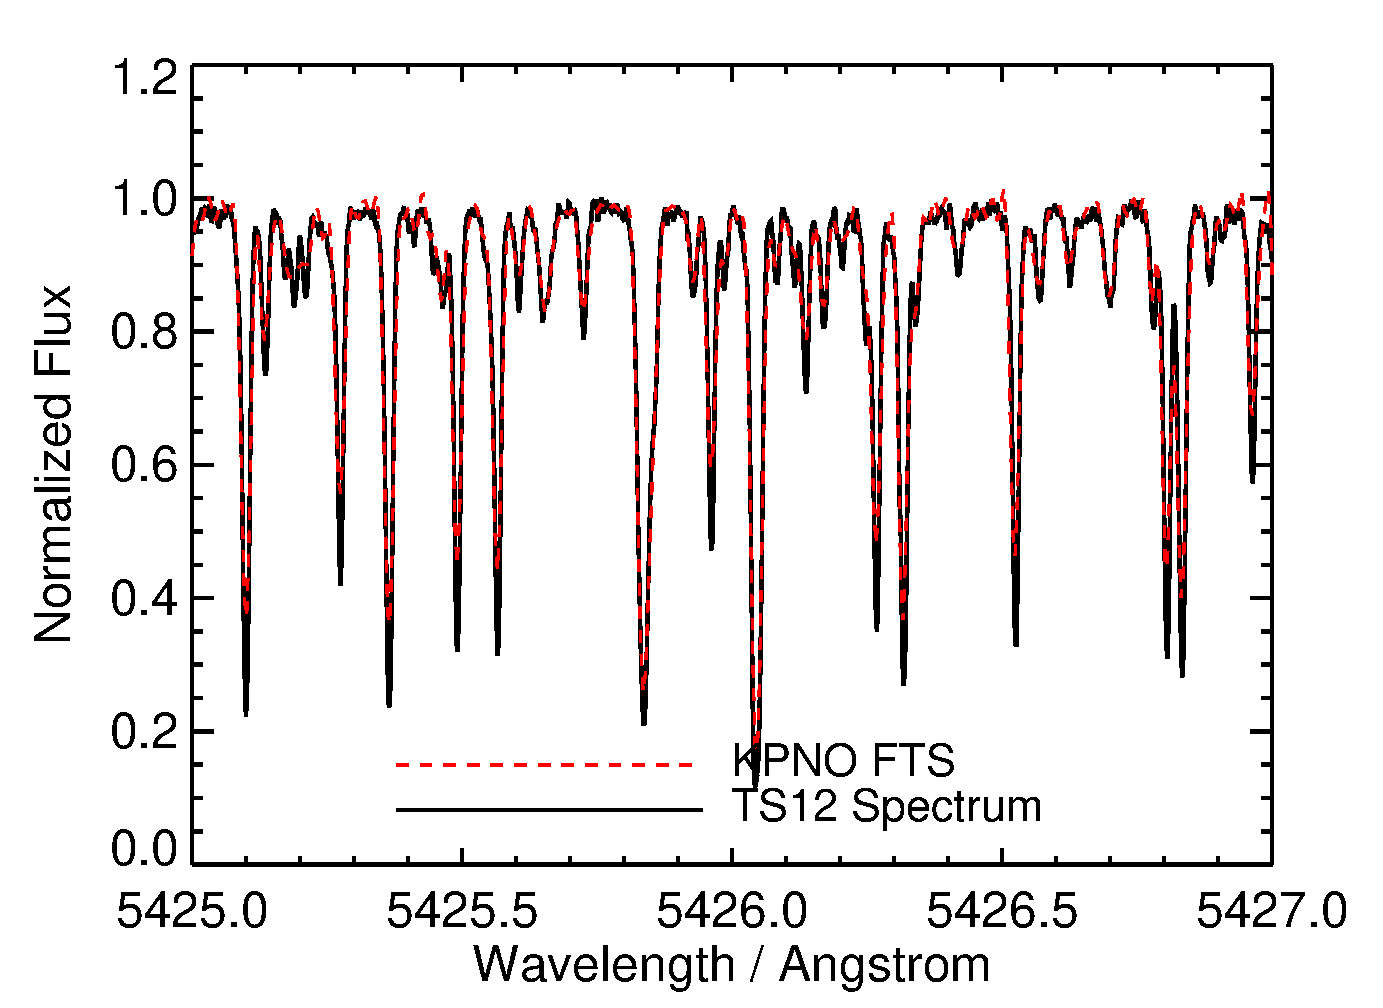
\includegraphics[angle=0.,scale=0.33]{het/chunk_5425A_original_sclrem.eps}
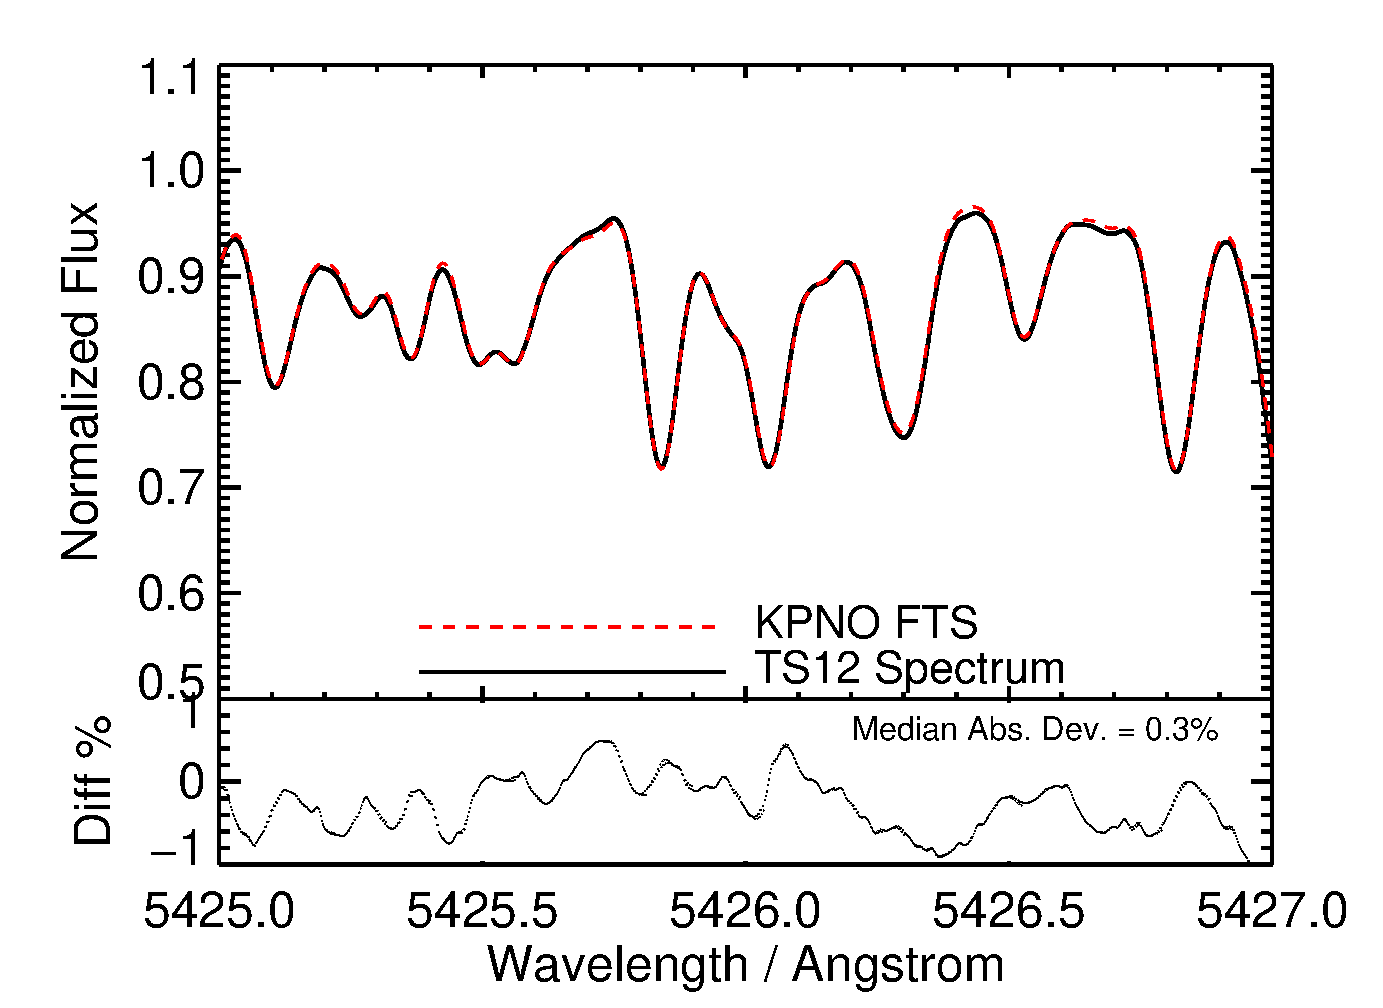
\includegraphics[angle=0.,scale=0.33]{het/chunk_5425A_60k_gaus_sclrem_diff.eps}
\caption{Comparison of the Sandiford iodine cell KPNO FTS spectrum and
  the spectrum taken with TS12. \textbf{Left:} Comparison of the two
  spectra in their native resolutions (both about
  $400,000$--$500,000$). \textbf{Right:} Comparison of the two spectra
  convolved down to about $60,000$ resolution, which is the resolution
  of typical iodine observations or radial velocity observations
  (star$+$iodine). Bottom panel shows the residuals in percentage of
  the TS12 spectrum minus the KPNO spectrum, with a median absolute
  deviation of 0.3\%.
  \label{fig:ts12}}
\end{figure*}
%----------------------------------------------------------------


%----------------------------------------------------------------
% Figure: TS12 spectrum vs. KPNO FTS scan, 60k, all, with residuals
\begin{figure}[!th]
\centering
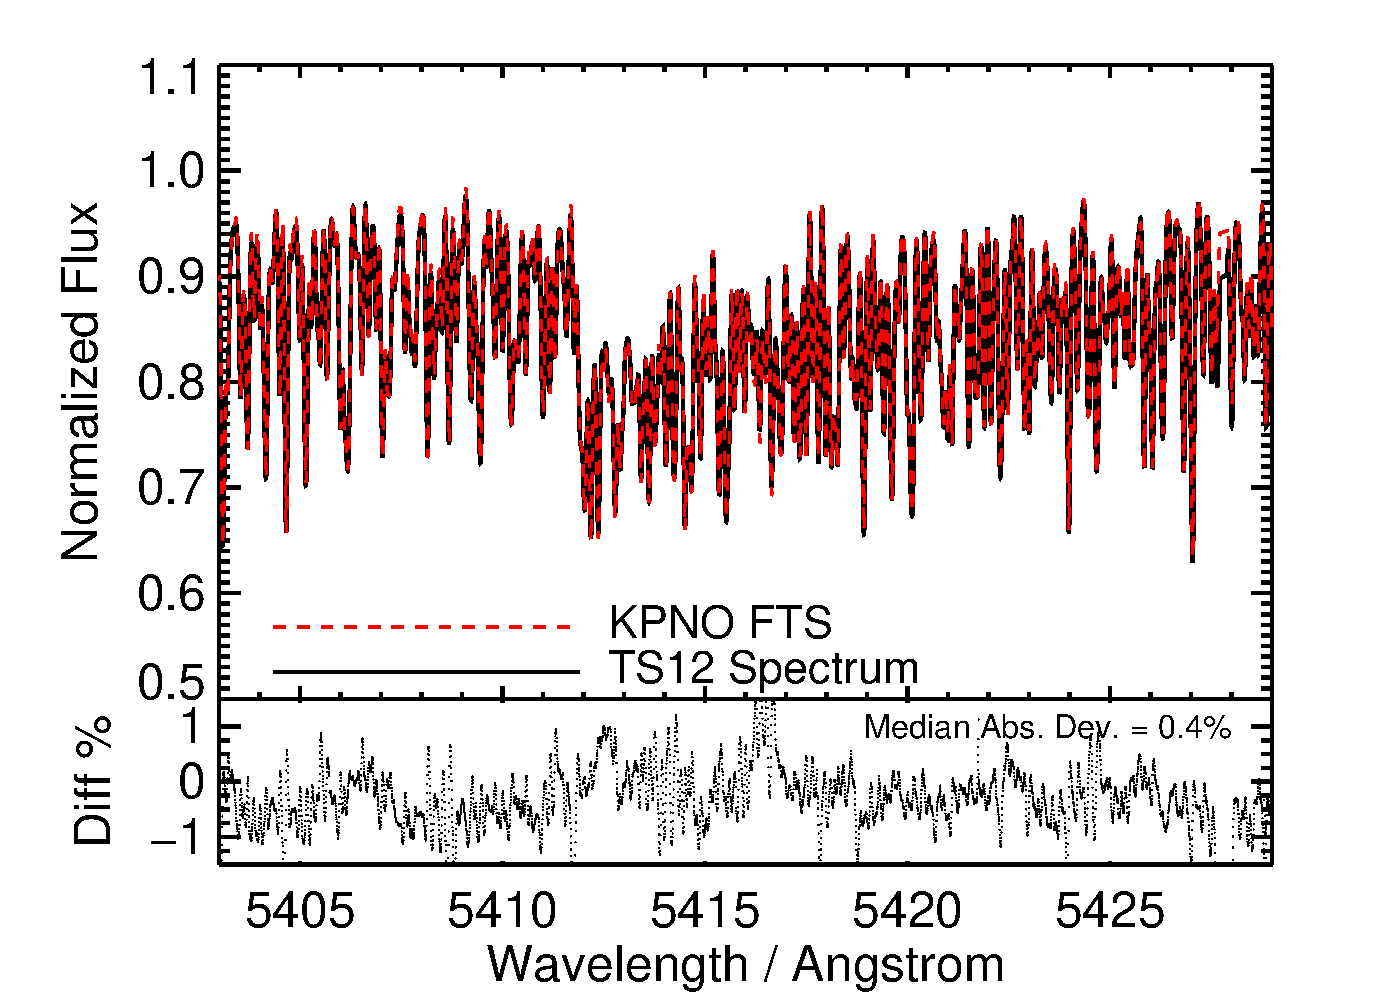
\includegraphics[angle=0.,scale=0.45]{het/all_60k_gaus_sclrem_diff.eps}
\caption{The same as the right panel of Figure~\ref{fig:ts12}, the
KPNO spectrum and the TS12 spectrum for the Sandiford cell both at
$60,000$, but for the entire $\sim$30\AA\ TS12 spectrum available. 
  \label{fig:60k_all}}
\end{figure}
%----------------------------------------------------------------


After demonstrated that we can use TS12 spectrum to validate FTS
scans, we performed our second TS12 run with the \het\ cell (and the
2.7m cell and the MINERVA cell). For
the 2.7m cell, its TS12 spectrum matches very well to its FTS atlas,
again (together with the 2.1m cell data from 2013) proving that TS12
is an appropriate tool for validating FTS atlases. For the HET/HRS
iodine cell, the results are very informative:

(1) Assuming that the \het\ cell temperature control was reliable
during our TS12 run (Phillip MacQueen from McDonald Observatory, who
built the cell and its enclosure, was at the TS12 run to set it up),
then temperature change on the order of 5--10$\degree$C in iodine cell
should induce a visible change in the absorption spectrum (right panel
of Figure~\ref{het:fig:tempchange}). On the other hand, the
temperature of the iodine gas in the cell was not at its set
temperature of $70\degree$C during the NIST scan (left panel of
Figure~\ref{het:fig:tempchange}). This could explain the difference
between \het\ cell's NIST scan and the KPNO scan. The NIST scan
appears to have stayed at higher than $70\degree$C the entire time
(one hypothesis is that the gas on the light path was heated up by the
ultra-luminous continuum lamp, while the glass container, which the
temperature probe was monitoring, stayed cool). The \keck\ cell was
also scanned at three different temperatures (50, 60, and
70$\degree$C) at KPNO in 1993, and there are also visible differences
between these three sets of scans.


%----------------------------------------------------------------
% HET cell spectral changes vs. temperature changes effects in TS12 and NIST scan
% plot made by
% ~/ExoPlanet-2010-2011/HET-HRS-IP/05-Iodine_FTS_investigation/compare_fts/explore_temp_change.pro and saved therein
\begin{figure}
\centering
\subfloat{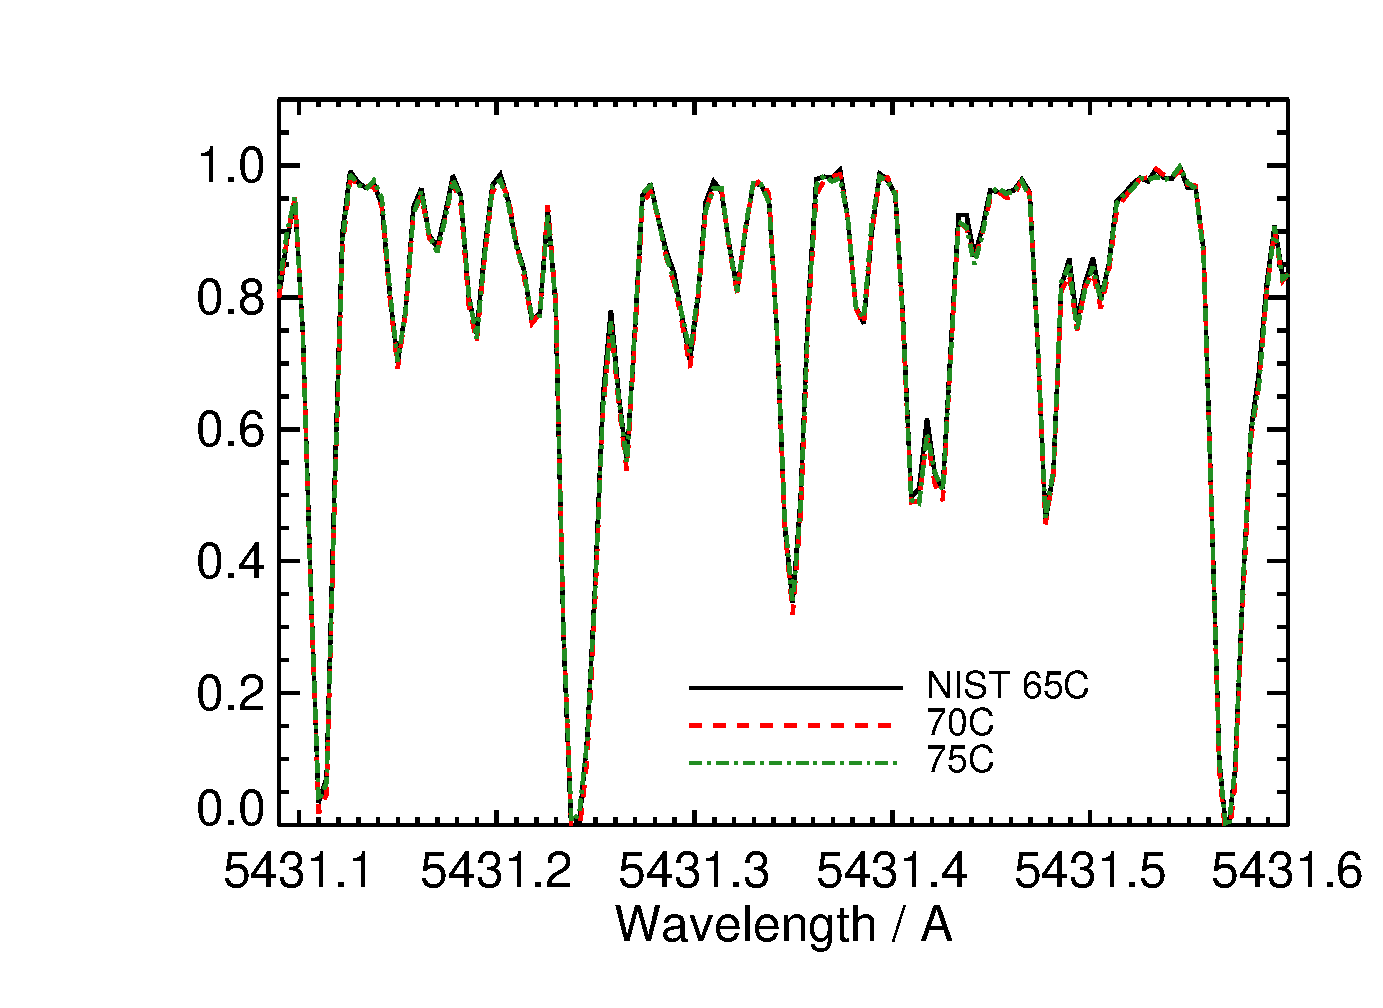
\includegraphics[scale=0.32]{het/nist_temp_change.eps}}
\subfloat{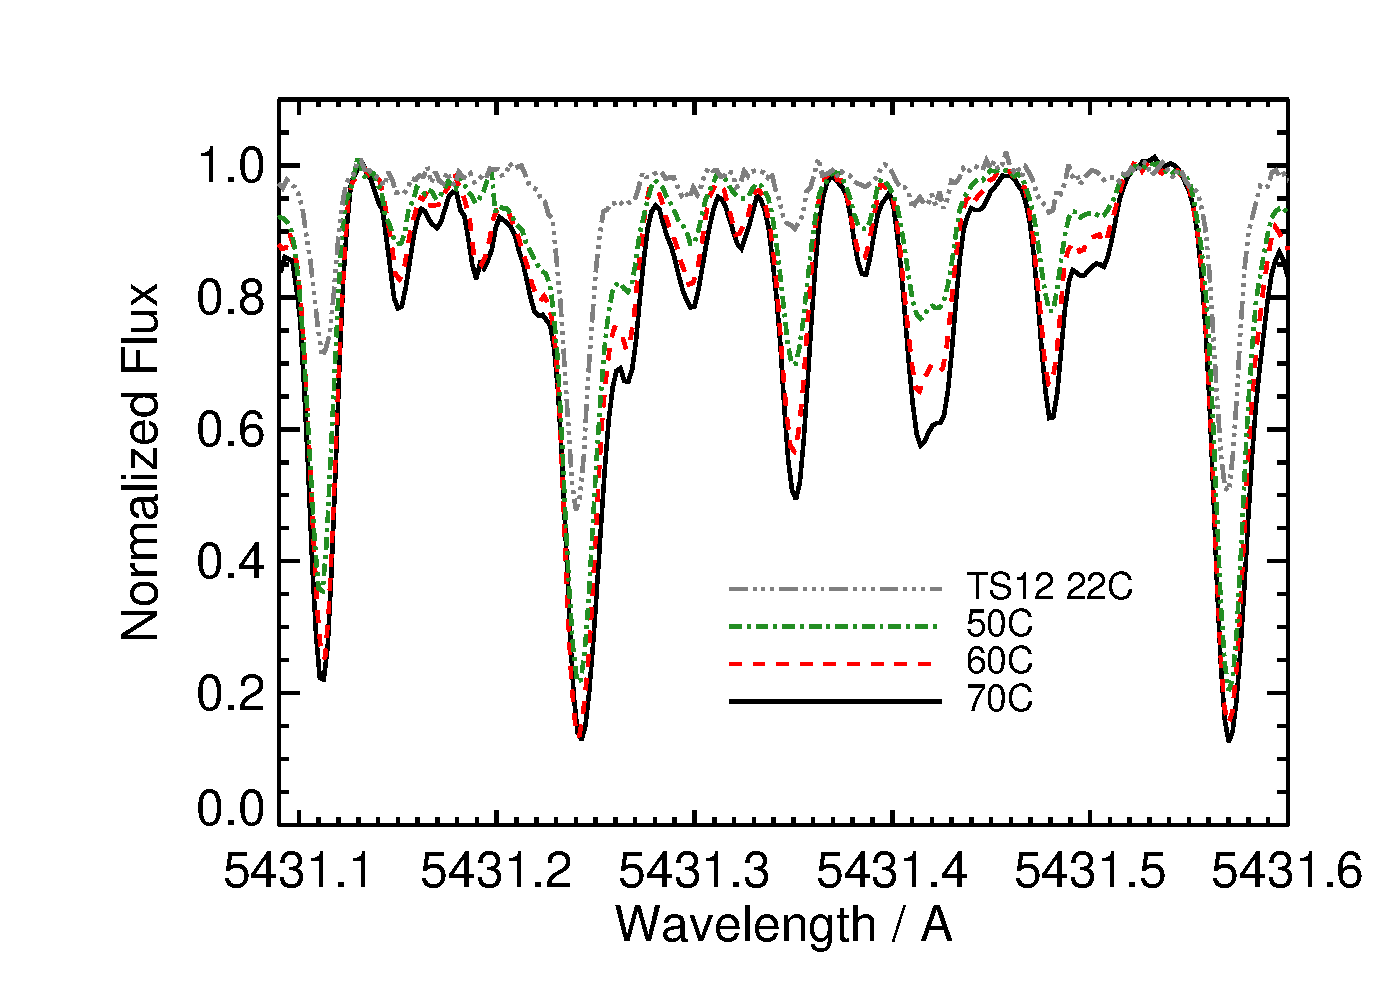
\includegraphics[scale=0.32]{het/ts12_temp_change.eps}}
\caption{{\bf Left:} \het\ cell NIST FTS scan at three different
temperatures. {\bf Right:} \het\ cell TS12 spectra at four different
temperatures for the same wavelength region, which, unlike the NIST
scans, shows significant difference when the temperature of the cell
changes by 10$\degree$C.
\label{het:fig:tempchange}}
\end{figure}
%----------------------------------------------------------------



(2) The TS12 spectrum at $70\degree$C matches better with the more
recent but potentially problematic NIST FTS atlas
(Figure~\ref{het:fig:hetts12}). This is completely unexpected and
contradicts with the assumptions and/or conclusions we lay out in
finding (1). The TS12 spectrum also does not match the FTS scan well
enough given the high SNR nature of both. Perhaps neither TS12 or the
NIST scan was at $70\degree$C. Or, perhaps the amount of iodine vapor
was somehow different. 


%----------------------------------------------------------------
% HET/HRS cell, TS12 vs KPNO vs NIST
% plot from ~/TS12/match_fts/figure/, made by plotcomp.pro
% grabbed from ~/ExoPlanet-2010-2011/Professional_Development/201402-NESSF/renewal/proposal/
\begin{figure}
\centering
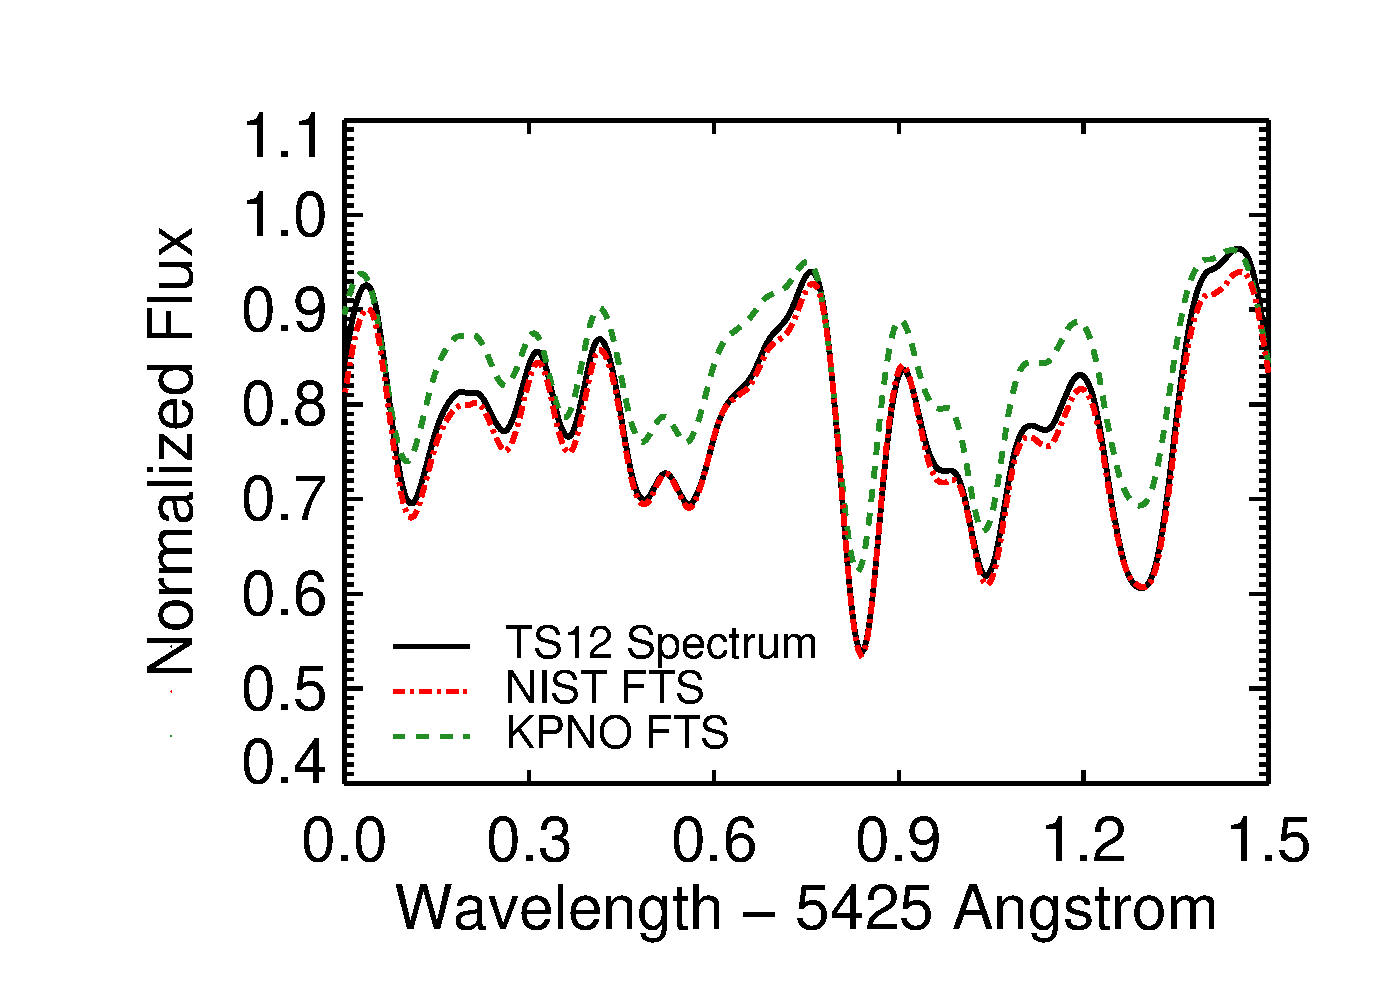
\includegraphics[scale=0.5]{het/het70_comp.eps}
\caption{TS12 spectrum (black solid line) vs.\ NIST FTS (red
  dotted-dashed) vs.\ KPNO FTS (green dashed) for the \het\ iodine
  cell at 70$\degree$C, all convolved down to a resolution of R $=$
  60k (the same as a typical \het\ observation) for comparison
  purposes. The TS12 spectrum matches the NIST FTS better, having
  deeper lines compared to the original KPNO FTS. The remaining
  difference between NIST FTS and the TS12 spectrum might be due to
  differences in cell temperatures or other changes with the cell. 
\label{het:fig:hetts12}}
\end{figure}
%----------------------------------------------------------------

These results prompted us to resolve for a second route to try to break
the tie: using synthetic iodine absorption spectra, which is described
in the next subsection.


%%%%%%%%%%%%%%%%%%%%%%%%%%%%%%%%%%%%%%%%%%%%%%%%%%%%%%%%%%%%%%%%%%%%%%%%%%%%%%%%%%%%%%%%%%%%%%%%%%%%
\subsection{Measuring iodine cell temperatures using synthetic Iodine spectra}

Using the TS12 spectra, we found that the temperature of the iodine
gas in the cell might not be the same one reported by the temperature
controller. However, we still could not break the tie between the KPNO
scan and the NIST scan for \het\ cell: the KPNO scan provides a better
fit to real observed data, but the TS12 spectrum shows us that the
NIST scan looks closer to the ``truth'' as defined by TS12. Nor did we
understand why the KPNO scan for the \keck\ cell works the best for
\het\ data.

To answer these questions, we have found\footnote{We are deeply
  grateful for Iouli Gordon for introducing IodineSpec5 to me
  during my visit at CfA.} a second venue that provides
reliable, ultra-high resolution, and wavelength calibrated iodine
atlas -- a theoretical code that computes synthetic iodine
transmission spectrum (at any specified temperature) based on both
physics and empirical calibrations (IodineSpec5;
\citealt{iodinespec5}). We emailed the authors and obtained the code,
which only runs on Windows machines. The direct output of the code
contains arrays of wave numbers and ``opacity'' ($\alpha$) for user-specified
iodine isotope mix (for our purposes we only add $^{127}I_2$),
temperature, wave number range, and line broadening kernel parameter
(we chose thermal/Gaussian). To use the output of IodineSpec5 to fit
an actual iodine absorption spectrum, there are two parameters:
gas temperature and a constant which scales with iodine molecule
column density, which we simply refer to as the column density hereafter.

Quickly comparing the NIST scan with the IodineSpec5 models reveals
that the NIST scan seems to be around 110$\degree$C, mostly based on
visually examining the line ratios
(Figure~\ref{het:fig:nisteyeball}). However, the synthetic iodine
spectrum and the FTS scans have different broadening kernels. In order
to ``fit'' the NIST scan with the synthetic spectra at various
temperatures, we convolved the NIST scan with a single Gaussian kernel
with $\sigma=0.0078$ (roughly at $R=$ 200,000 to try to match the
\keck\ cell KPNO scan for comparison and illustration
purposes). Except for the \keck\ scan, we did the same to lower the
resolution of other FTS scans or TS12 spectra when using IodineSpec5
to find out their temperatures. There are three four parameters in our
fit: temperature, column density, resolution ($\sigma$ for the single
Gaussian kernel to convolve the synthetic spectrum with), and a
wavelength shift. We first optimized the column density, $\sigma$, and
the wavelength shift while fixing the temperature (using L-M
least-$\chi^2$ fitter using {\tt mpfitfun} package in IDL), and then
we compare the goodness of fit of each model at different temperatures
to determine which temperature best describes the FTS scan or TS12
spectrum. The reason for this two-step optimization is because we have
to generate the IodineSpec5 model spectra on a discrete temperature
grid.


%----------------------------------------------------------------
% HET/HRS cell, IodineSpec5 2 temperatures vs. NIST, and KPNO
% plot from ~/ExoPlanet-2010-2011/IodineSpec5/, made by plots_general.pro
\begin{figure}
\centering
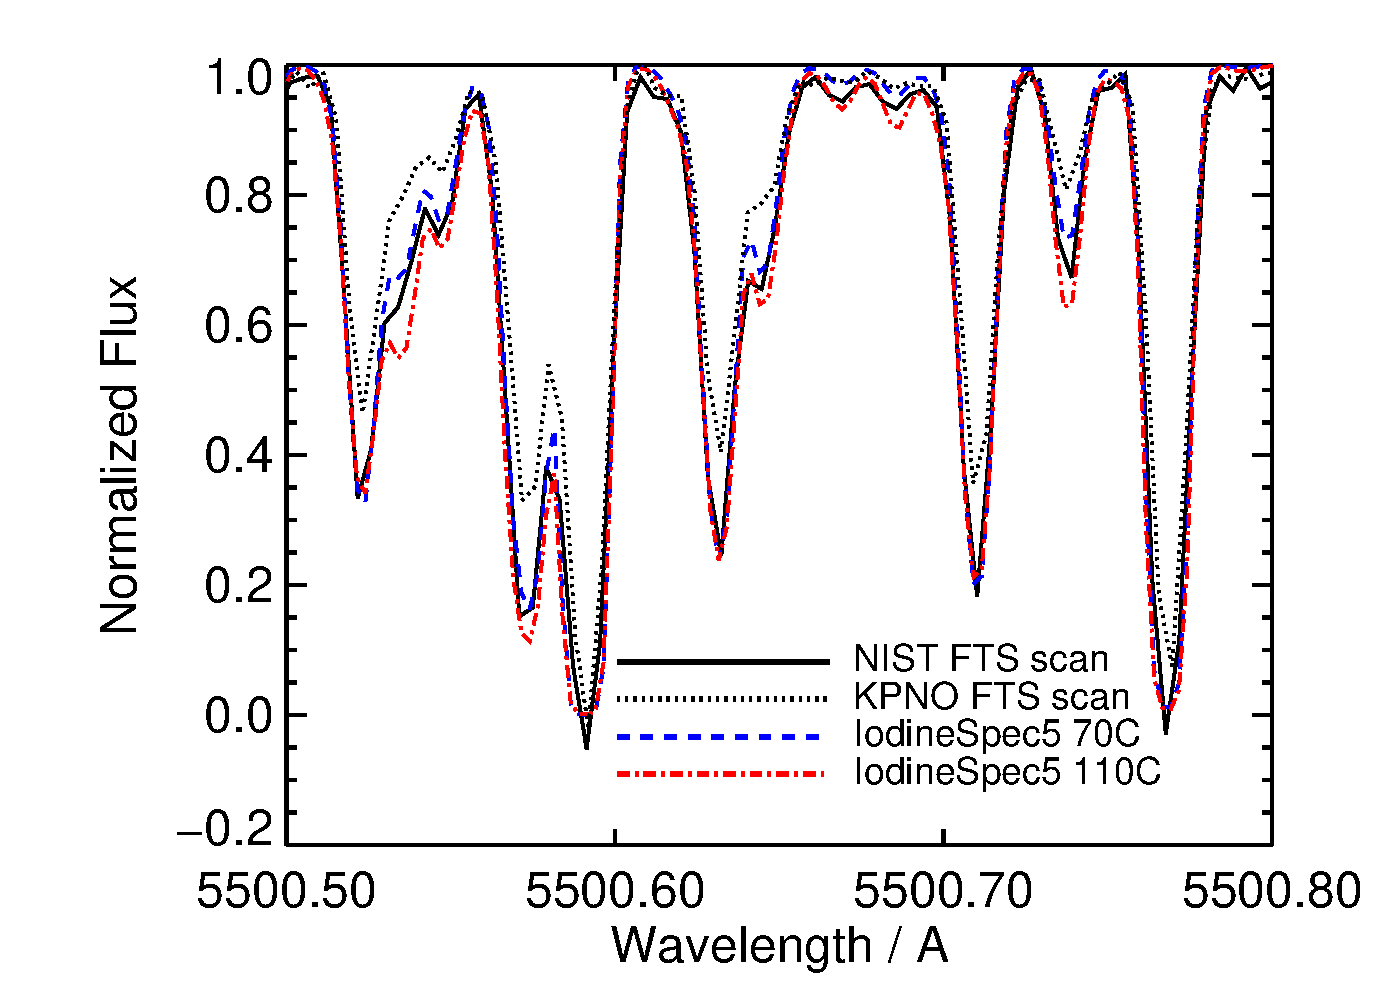
\includegraphics[scale=0.5]{het/HET_NIST_temp.eps}
\caption{NIST FTS (black solid lines) and KPNO FTS (black dotted
lines) compared with theoretically computed iodine lines at
70$\degree$C (blue dashed) and 150$\degree$C (red dotted-dashed). All
spectra are at their original resolution. There are two free
parameters for the theoretical lines: temperature and iodine column
density. For this plot, we optimized the iodine column density for the
theoretical lines at both temperatures to try to match the NIST FTS. As
illustrated, neither temperature can produce a good match, and the
best temperature is around 110$\degree$C. Note that the
theoretical lines and the NIST FTS have different broadening
kernels. The NIST and KPNO FTS scans probably differ in both optical
depth and cell temperature.
\label{het:fig:nisteyeball}}
\end{figure}
%----------------------------------------------------------------

We first fitted the \keck\ cell KPNO FTS scan, whose temperature is
known (50$\degree$C) and reliable. We also know that this FTS scan is
probably very trust-worthy since \keck\ iodine atlas fits the data
very well, as described in the previous subsection. Choosing a region
where it contains temperature-sensitive lines, we found the best-fit
temperature for the \keck\ KPNO scan is 55$\degree$C, although
synthetic spectra ranging from 40-70$\degree$C all fit the data
almost equally well and they are hard to distinguish (column density
and temperature are highly degenerate parameters). 

We then fitted the NIST scan, which has the highest SNR and
resolution among all FTS scans or TS12 spectra (we also have a rough
idea about its temperature). The results are shown in
Figure~\ref{het:fit:nistfit}, where the top panel shows the best-fit
models at different temperatures, and the bottom panel compares the
NIST scan with its the best-fit model at 110$\degree$C, the KPNO scan,
and the \keck\ cell KPNO scan. 


%----------------------------------------------------------------
% NIST scan fit by IodineSpec5 and comparison with FTS
% plot made by
% ~/ExoPlanet-2010-2011/HET-HRS-IP/05-Iodine_FTS_investigation/compare_fts/fit_temp_change.pro and saved therein
\begin{figure}
\centering
\subfloat{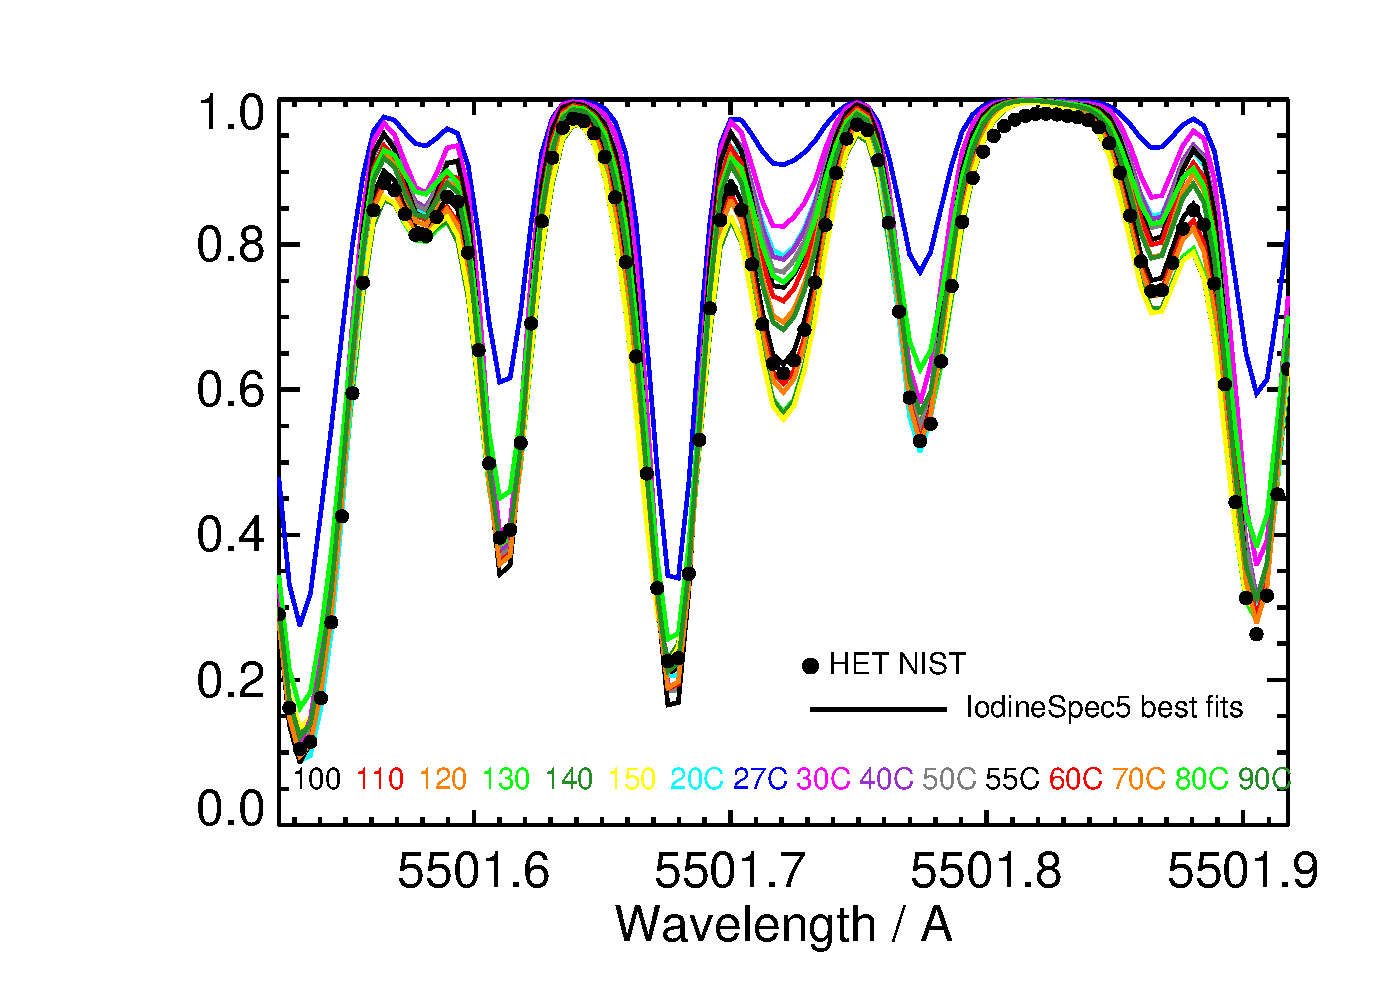
\includegraphics[scale=0.5]{het/hetnist_bestfits.eps}}\
\subfloat{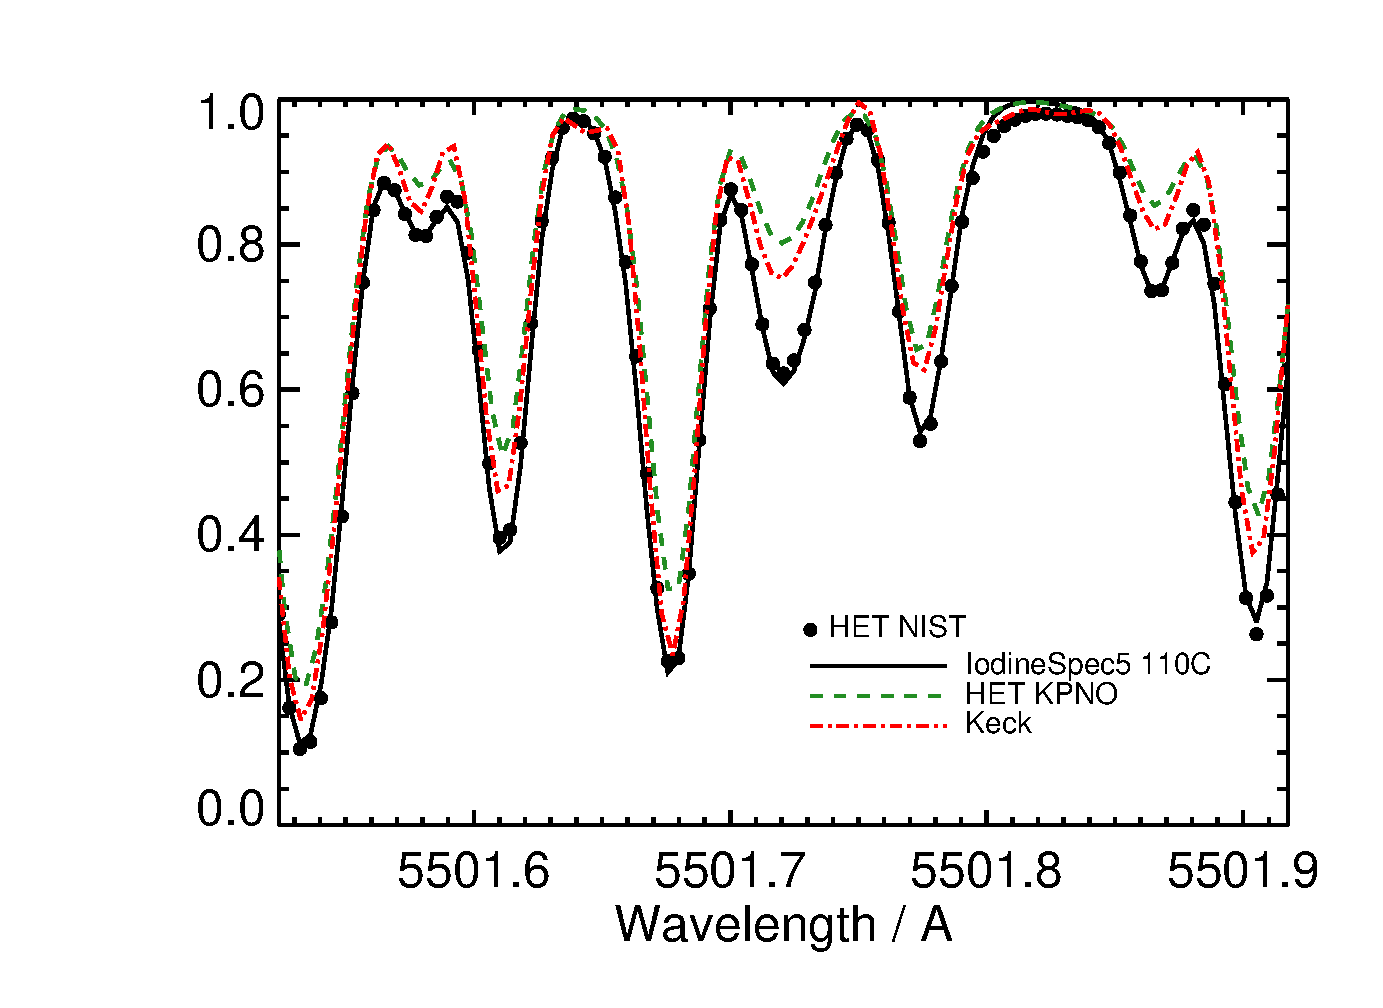
\includegraphics[scale=0.5]{het/hetnist_compWithOthers.eps}}
\caption{{\bf Top:} Fitting \het\ NIST scan (black dots; temperature
set at 70$\degree$C) with IodineSpec5 synthetic iodine lines at
various temperatures and column densities. {\bf Bottom:} The \het\
NIST scan (black dots) overplotted with the best-fit IodineSpec5 model
(black solid line; at 110$\degree$C) and the \het\ cell and \keck\ 
cell KPNO scans. All spectra in both panels are convolved down to a
resolution of 200,000 (roughly \keck\ KPNO FTS scan resolution) to
wash out the intrinsic IP difference between FTS scan (sinc function
IP) and the synthetic spectrum (only natural broadening IP models).
\label{het:fig:nistfit}}
\end{figure}
%----------------------------------------------------------------

When we tried to fit the \het\ KPNO scan, the high degeneracy between
column density and temperature hindered us from getting an accurate
estimate for the temperature. Models in 40-80$\degree$C appear to fit
equally well with varying column densities. However, only the fit at
$70\degree$C has the same column density as the best-fit value derived
from the NIST fit. We thus fixed the column
density in our fits for \het\ KPNO scan, and (unsurprisingly) the best-fit
temperature came out to be $70\degree$C. Therefore, we conclude that
the NIST scan was indeed at a different gas temperature, and the old
KPNO scan seems to be at the right temperature.

But how about the TS12 spectrum? Again, using the best-fit column
density derived from our NIST and KPNO fits, we estimated the
temperatures for the TS12 spectra (supposedly) at 50, 60, and
70$\degree$C. The best-fit temperature turns out to be 55$\degree$C
for claimed 50$\degree$C TS12 spectrum, 80$\degree$C for the
60$\degree$C one, and 100$\degree$C for the 70$\degree$C one. The
results fitting for the ``70$\degree$C'' TS12 spectrum are in
Figure~\ref{het:fig:ts12fit}.  


%----------------------------------------------------------------
% TS12 fit by IodineSpec5 and comparison with FTS
% plot made by
% ~/ExoPlanet-2010-2011/HET-HRS-IP/05-Iodine_FTS_investigation/compare_fts/fit_temp_change.pro and saved therein
\begin{figure}
\centering
\subfloat{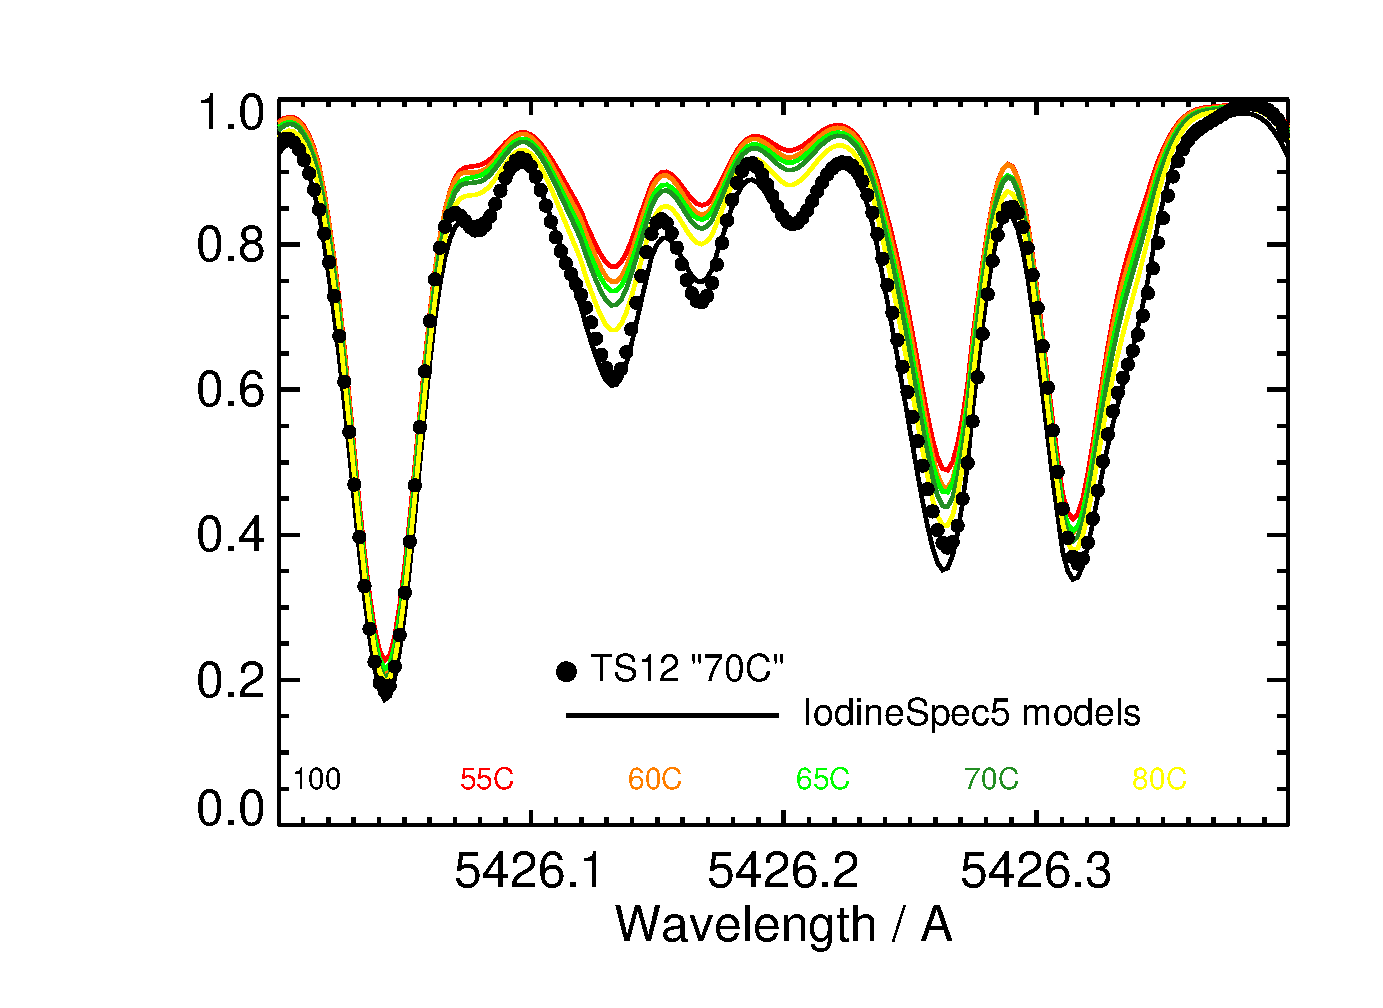
\includegraphics[scale=0.5]{het/ts12_70_bestfits.eps}}\
\subfloat{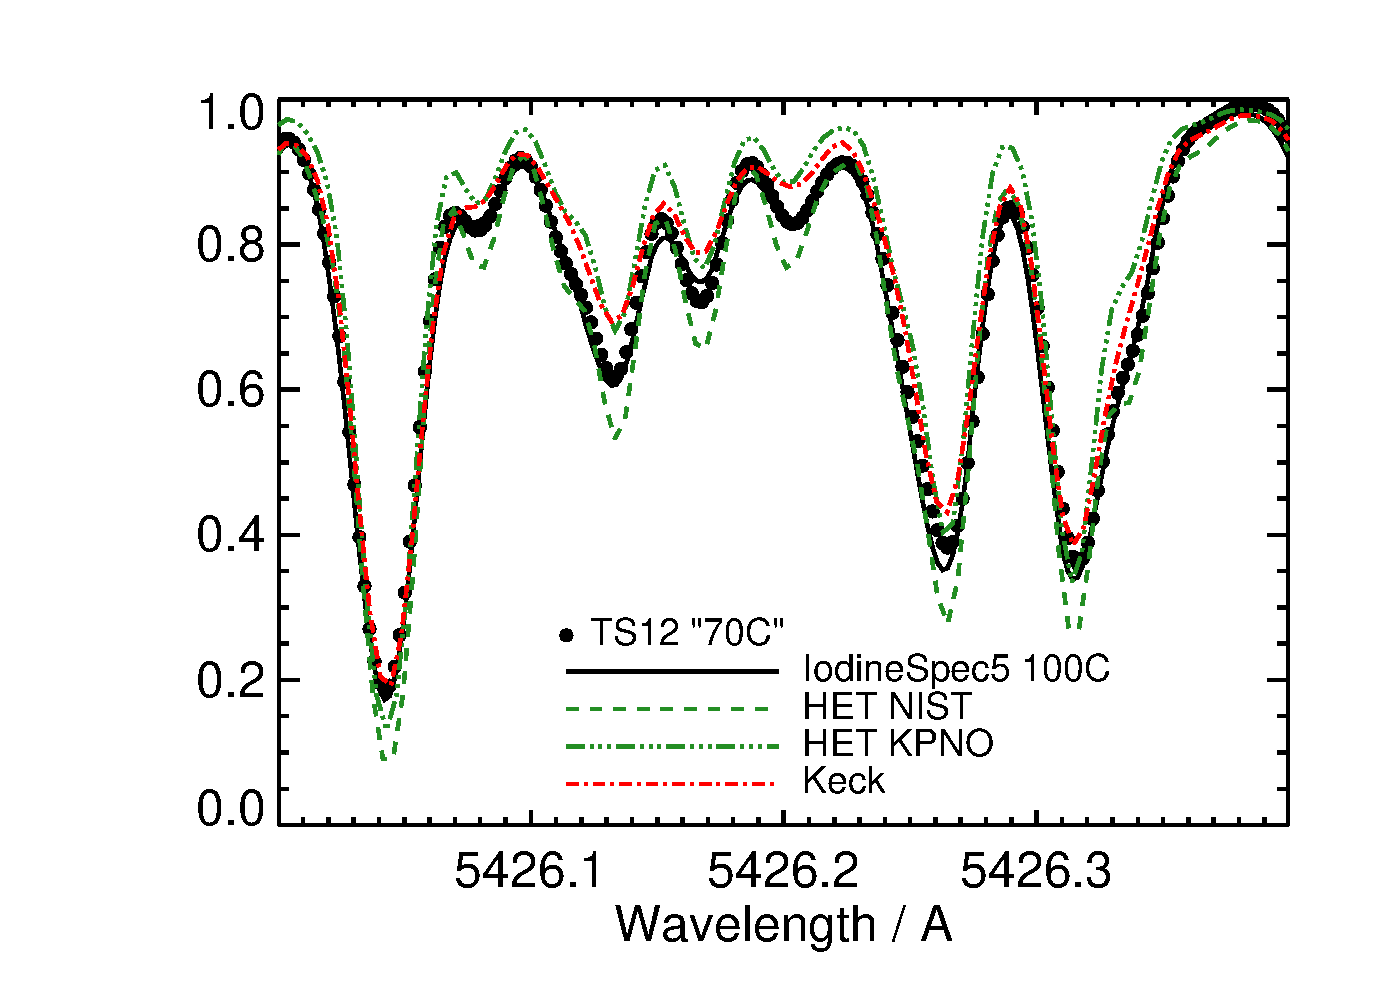
\includegraphics[scale=0.5]{het/ts12_70_compWithFTS.eps}}
\caption{{\bf Top:} Fitting the TS12 spectrum (temperature set at
70$\degree$C; black dots) with IodineSpec5 models, with fixed column
density derived from best fits using \het\ KPNO and NIST scans. {\bf
Bottom:} The best-fit temperature for the TS12 spectrum is about
100$\degree$C (black solid). It is clearly at a lower temperature than
the NIST scan (green dashed) but at a higher one than the KPNO one
(green dotted-dashed). Again, all spectra in both panels are convolved
down to $R=$ 200,000.
\label{het:fig:ts12fit}}
\end{figure}
%----------------------------------------------------------------

These findings on \het\ cell temperatures could explain the fits to
real data. If the \het\ cell was kept at a higher temperature (e.g.,
$\sim 100\degree$C) instead of $70\degree$C when it was in active use
for precise RV calibration (despite what the temperature control
reported), or if the actual temperature of the gas in the cell changes
over time, then the KPNO scan, which was done at $70\degree$C,
certainly cannot fit the observed data and provide precise
calibrations to measure RVs to the level of \keck, which has a precise
iodine atlas. Looking at the bottom panel of
Figure~\ref{het:fig:ts12fit}, it is not hard to imagine why the \keck\
cell scan provides the best fits to \het\ data
(Figure~\ref{fig:lampi2fit}) -- if the gas temperature is between 70
and 110$\degree$C during actual observations (and perhaps more often
closer to 70$\degree$C), then an iodine atlas which has line depths in
between the KPNO and the NIST scans would provide a better fit, which
the \keck\ scan happens to satisfy.

We believe that the difference between the iodine atlas and reality as
a result of temperature changes or differences is the dominant factor
behind \het's under-performance in RV precision compared with
\keck. We outline potential solutions to improve the RV precision of
\het\ archival data and our recommendations for the new HRS in the
next section.


%%%%%%%%%%%%%%%%%%%%%%%%%%%%%%%%%%%%%%%%%%%%%%%%%%%%%%%%%%%%%%%%%%%%%%%%%%%%%%
%\section{The Investigation on Modal Noise}
  
